% ****** Start of file apssamp.tex ******
%
%   This file is part of the APS files in the REVTeX 4.1 distribution.
%   Version 4.1r of REVTeX, August 2010
%
%   Copyright (c) 2009, 2010 The American Physical Society.
%
%   See the REVTeX 4 README file for restrictions and more information.
%
% TeX'ing this file requires that you have AMS-LaTeX 2.0 installed
% as well as the rest of the prerequisites for REVTeX 4.1
%
% See the REVTeX 4 README file
% It also requires running BibTeX. The commands are as follows:
%
%  1)  latex apssamp.tex
%  2)  bibtex apssamp
%  3)  latex apssamp.tex
%  4)  latex apssamp.tex
%
\documentclass[%
 reprint,
%superscriptaddress,
%groupedaddress,
%unsortedaddress,
%runinaddress,
%frontmatterverbose, 
%preprint,
%showpacs,preprintnumbers,
nofootinbib,
%nobibnotes,
%bibnotes,
 amsmath,amssymb,
 aps,
%pra,
%prb,
%rmp,
%prstab,
%prstper,
floatfix,
]{revtex4-1}

\RequirePackage{luatex85}
\usepackage[compat=1.1.0]{tikz-feynman}
\usepackage{contour}
\usepackage{slashed}
\usepackage{amssymb}
\usepackage{graphicx}% Include figure files
\usepackage{dcolumn}% Align table columns on decimal point
\usepackage{bbm}% bold math
\usepackage{siunitx}
\usepackage{natbib}
%\usepackage{hyperref}% add hypertext capabilities
%\usepackage[mathlines]{lineno}% Enable numbering of text and display math
%\linenumbers\relax % Commence numbering lines

%\usepackage[showframe,%Uncomment any one of the following lines to test 
%%scale=0.7, marginratio={1:1, 2:3}, ignoreall,% default settings
%%text={7in,10in},centering,
%%margin=1.5in,
%%total={6.5in,8.75in}, top=1.2in, left=0.9in, includefoot,
%%height=10in,a5paper,hmargin={3cm,0.8in},
%]{geometry}
\newcommand*{\ATLASLATEXPATH}{latex/}

\usepackage{\ATLASLATEXPATH atlasphysics}

\DeclareMathOperator{\Lagr}{\mathcal{L}}
\DeclareMathOperator{\melement}{\mathcal{M}}
\DeclareMathOperator{\del}{\partial}
\DeclareMathOperator{\D}{\mathcal{D}}
\DeclareMathOperator{\F}{\mathcal{F}}
\DeclareMathOperator{\G}{\mathcal{G}}
\DeclareMathOperator{\Ham}{\mathcal{H}}
\DeclareMathOperator{\J}{\mathcal{J}}
\DeclareMathOperator{\BigO}{\mathcal{O}}
\DeclareMathOperator{\Proj}{\mathcal{P}}
\DeclareMathOperator{\V}{\mathcal{V}}
\DeclareMathOperator{\BigZ}{\mathcal{Z}}
\DeclareMathOperator{\Tr}{Tr}
\DeclareMathOperator{\mytab}{\,\,\,\,\,\,\,\,\,\,\,\,\,\,\,\,}
\newcommand\underrel[2]{\mathrel{\mathop{#2}\limits_{#1}}}


\begin{document}

\preprint{APS/123-QED}

\title{Electroweak Symmetry Restoration}% Force line breaks with \\
\thanks{PHYS 7240 (Advanced Statistical Mechanics) Term Paper}%

\author{Jeff Ouellette}
 \altaffiliation[]{Physics Department, University of Colorado Boulder}%Lines break automatically or can be forced with \\
 \email{\\jeffrey.ouellette@colorado.edu}
\affiliation{%
 University of Colorado Boulder\
}%

\date{\today}% It is always \today, today,
             %  but any date may be explicitly specified

\begin{abstract}
The discovery of the Higgs' boson in 2012 represented the final necessary discovery that solidified electroweak theory as the proper description of both the electromagnetic and weak forces at high energies.
At its heart lies the spontaneous breaking of gauge symmetry by the Higgs' field, which acquires a nonzero vacuum expectation value (a condensate).
At zero temperature, the condensate is fixed by the tree level Lagrangian and its magnitude has been measured in experiment.
But at high enough temperatures, statistical fluctuations in the Goldstone modes are expected to lead to symmetry restoration.
In this paper we review how such interactions provide temperature dependence to the effective potential.
We calculate the thermal effective potential $\V$ to one-loop order in different example models to understand the effects of couplings to different fields, citing particular differences between scalars/vectors (bosons) and spinors (fermions).
A general phase transition mechanism is identified at high temperatures in which the electroweak symmetry is restored.
The order of the phase transition is important in cosmology, as a first order transition would provide a baryogenesis mechanism, therefore explaining the matter-antimatter asymmetry.
Equipped with the thermal effective potential, we demonstrate that the phase transition is not likely to be strongly enough first order to allow successful electroweak baryogenesis within the standard model.
\end{abstract}

\pacs{Valid PACS appear here}% PACS, the Physics and Astronomy
                             % Classification Scheme.
%\keywords{Suggested keywords}%Use showkeys class option if keyword
                              %display desired
\maketitle

%\tableofcontents

\section{\label{sec:intro}Introduction}
As late as the 1960's, the best theory of a weak nuclear force was the vector-minus-axial interaction, which was successful in describing low-energy experiment results.
To describe this force at high energies, physicists turned to Yang-Mills theories based on the ``smallest'' possible gauge group $SU(2)$.
While a compelling theory, it came bundled with a crucial flaw by which the force-carrying particles required masses -- large masses -- to make the force very short-ranged at low energies.
Yang-Mills theory explicitly disallows gauge boson mass terms in the underlying theory, as these break gauge invariance for $N\geq 2$ \cite{sher89}.

Two extensions of the model were identified to resolve this issue.
The first required the $SU(2)$ gauge group be packaged with a $U(1)$ gauge group; electromagnetism was already known to have $U(1)$ symmetry and was identified as the appropriate candidate.
This led to the concept of ``electroweak unification'', where both the electromagnetic and weak forces could be understood in the context of a single model.
The second ingredient famously proposed an additional scalar field $\Phi$ to be coupled to the $SU(2)$ gauge field.
This so-called Higgs' field was to live in the \textbf{2} (doublet) representation of $SU(2)$ and transform covariantly under both gauge groups, with covariant derivative $D_\mu \Phi = \left(\del_\mu + igT_iW^i_\mu + \frac{i}{2}g'B_\mu\right)\Phi$, where $T_i=\sigma_i/2$ are the $SU(2)$ generators and $g$ and $g'$ are the respective coupling constants for weak isospin (gauge fields $W^a_\mu$) and weak hypercharge (gauge field $B_\mu$).
Most importantly, $\Phi$ was allowed to self-interact through a quartic vertex, providing it a mechanism to acquire a nonzero vacuum expectation value.
Putting these elements together, the Lagrangian for such a model was written as:
\begin{equation}
\begin{split}
    \Lagr_\text{EW}= &-\frac{1}{4}W^{\mu\nu}_a W^a_{\mu\nu} - \frac{1}{4}B^{\mu\nu}B_{\mu\nu} \\ &+ \left|D_\mu \Phi\right|^2-\lambda\left(|\Phi|^2-\frac{v^2}{2}\right)^2.
\end{split}
\label{eq:smlagr}
\end{equation}
A typical representation of $\Phi$ is given by \cite{quiros99}
\begin{equation}
    \Phi = \begin{pmatrix} \chi_1 + i\chi_2 \\ \frac{1}{\sqrt{2}}\left(\phi_c + h + i\chi_3\right)\end{pmatrix}
\end{equation}
where $\chi_i$ are the degrees of freedom eaten by the $W_a^\mu$ bosons, $h$ is the ``Higgs' boson'' field, and $\phi_c$ is the classical Higgs' field (referred to as the ``condensate'' or the vacuum expectation value).
At zero temperature, the $\Phi$ field tries to minimize the effective potential term and spontaneously breaks the $SU(2)$ symmetry to acquire a vacuum expectation value (VEV)
The VEV is described in mean-field theory \cite{dj74}
\begin{equation}
    \frac{d\V}{d\phi_c} = 0
\end{equation}
where $\V$ is the potential energy; the solution is clearly $\phi_c^2 = v^2$.
After $\V$ is minimized with respect to the VEV, the covariant derivative on $\Phi$ converts the $\phi_c$ terms to mass terms for gauge fields.
This can be seen by plugging in a constant $\Phi = \begin{pmatrix} 0 \\ \phi_c \end{pmatrix}$ to the covariant derivative term:
\begin{widetext}
\begin{equation}
\begin{split}
    \left(D_\mu\Phi\right)^\dag D^\mu\Phi &= \begin{pmatrix} 0 & \phi_c \end{pmatrix} \left(\overleftarrow{\del_\mu} - i\frac{g}{2}W_\mu^i\sigma_i-i\frac{g'}{2}g'B_\mu \right) \left(\overrightarrow{\del^\mu} + i\frac{g}{2}W_j^\mu\sigma^j+i\frac{g'}{2}g'B^\mu\right) \begin{pmatrix} 0 \\ \phi_c \end{pmatrix} \\
    &= \frac{1}{4}\begin{pmatrix} 0 & \phi_c \end{pmatrix} \left(gW_\mu^i\sigma_i + g'B_\mu\right)\left(gW^{\mu j}\sigma_j + g'B^\mu\right) \begin{pmatrix} 0 \\ \phi_c \end{pmatrix} \\
    &= \frac{1}{4}\left[g^2 W_\mu^iW^{\mu j} \begin{pmatrix} 0 & \phi_c \end{pmatrix} \sigma_i\sigma_j \begin{pmatrix} 0 \\ \phi_c \end{pmatrix} + 2gg' B_\mu W^{\mu i} \begin{pmatrix} 0 & \phi_c \end{pmatrix} \sigma_i \begin{pmatrix} 0 \\ \phi_c \end{pmatrix} + g'^2B_\mu B^\mu \phi_c^2 \right] \\
    &= \frac{1}{4}\left[g^2\phi_c^2 W_\mu^i W^{\mu j}\left(\delta_{ij}-i\epsilon_{ijk}\delta_{k3}\right) - 2gg'\phi_c^2 B_\mu W^{\mu i}\delta_{i3} + g'^2 \phi_c^2 B_\mu B^\mu\right] \\
    &= \frac{\phi_c^2}{4}\left[g^2 W_\mu^iW^{\mu i} - 2gg'B_\mu W^\mu_3 + g'^2 B_\mu B^\mu\right].
\end{split}
\end{equation}
\end{widetext}
The physically observable electroweak bosons $\gamma, W, \& Z$ are defined through rotations of these fields and acquire their mass through this mechanism.
In the process, three degrees of freedom (the three Goldstone bosons $\chi_i$) are transferred from $\Phi$ to the longitudinal components of three linear combinations of $W_\mu^a$ and $B_\mu$.
One of the charge-neutral linear combinations is left without a longitudinal component, making it massless -- this is the photon $A_\mu$.
This mechanism miraculously gives the $W^\pm$ and $Z$ bosons masses without explicitly breaking the $SU(2)$ symmetry in the underlying microscopic theory.

One might then ask the question: what happens at high temperatures?
If the $\Phi$ field is surrounded by a thermal bath at temperatures of order the electroweak scale ($T\sim v=246~\GeV$), naively we should expect that these fields will start fluctuating, since they must contain a large amount of energy.
Eventually, the $\phi_c$ field should be fluctuating quite a lot.
From the point of view of the ordered phase, this would be indicative of a phase transition occurring around temperatures such that $\delta\phi_c/\phi_c \sim 1$.

But compared with, for example, a typical Landau theory of a ferromagnet, immediately we notice a major difference in the structure of the model: there is no explicit temperature dependence on the couplings.
The mean field theory analysis of the field $\phi_c$ returns a constant minimum at $v^2/2$, regardless of the ambient temperature.
This is in contradiction with our expectation; how can there be a phase transition if temperature doesn't appear in the theory?
Through simplified examples, we will see that the temperature dependence in model parameters emerges through interactions between the condensate and the medium.
Generally speaking, the condensate can interact via loop diagrams with the fields it couples to, which corrects the effective potential perturbatively in the quartic coupling.
To understand the effect of these corrections, we turn to scalar field theory.

\section{\label{sec:ftqft}Thermal Field Theory Primer}
Before diving into the statistical physics, it is important to cite the differences between finite temperature quantum mechanics and finite temperature quantum field theory.
In textbook quantum statistical mechanics, we start by defining the density matrix $\rho=\sum_{i}p_i\left|\psi_i\right>\left<\psi_i\right|=\exp\left(-\beta H\right)$.
%\footnote{In this paper we will work within the canonical ensemble, $\mu=0$.}
Expectation values of operators at finite temperature can then be calculated via the ``thermal trace'' $\left<A\right> = \frac{\Tr \rho A}{\Tr \rho}$.
In particular, we define the partition function via the identity operator: $Z = \left<1\right> = \Tr \rho$.
Then we can calculate equilibrium thermodynamic correlation functions by taking appropriate derivatives of $\ln Z$.

Now lets work within a quantum field theory, where the operators are promoted to fields.
Correlation functions at finite temperature, denoted by $\left<...\right>_\beta$, can be calculated similarly, but now depend on the position in space and time.
In particular, suppose we have a quantum field $\phi(x, t)$.
Then the key difference between studying the dynamics of $\phi$ at $T=0$ and $T\neq 0$ can be summarized in the correlation function \cite{yang11}
\begin{equation}
    \left<\phi(x,t)\phi(y,0)\right>_\beta = \frac{1}{Z} \Tr \left(e^{-\beta H}\phi(x,t)\phi(y,0)\right)
    %&= \frac{1}{Z} \left(\phi(x,t)e^{-\beta H}e^{\beta H}\phi(y,0)e^{-\beta H}\right).
\end{equation}
We will insert the identity $\mathbbm{1}=e^{-\beta H}e^{\beta H}$ and use the cyclic property of the trace $\Tr AB = \Tr BA$.
Note also that in the Heisenberg picture the operator $\phi$ evolves in time,
\begin{equation}
    \phi(y,-i\beta) = e^{i\left(-i\beta H\right)}\phi(y,0)e^{-i\left(-i\beta H\right)}.
\end{equation}

\begin{widetext}
\begin{equation}
\begin{split}
    \frac{1}{Z} \Tr \left(e^{-\beta H}\phi(x,t)\phi(y,0)\right) &= \frac{1}{Z} \Tr \left(\phi(x,t)e^{-\beta H}e^{\beta H}\phi(y,0)e^{-\beta H}\right) \\
    &= \frac{1}{Z} \Tr \left(\phi(x,t)e^{-\beta H} e^{i(-i\beta)H} \phi(y, 0)e^{-i(-i\beta)H}\right) \\
    &= \frac{1}{Z} \Tr \left(e^{-\beta H} \phi(y, -i\beta) \phi(x,t)\right) \\
    &= \left<\phi(y, -i\beta)\phi(x, t)\right>_\beta
\end{split}
\end{equation}
\end{widetext}

So we end up with the Kubo-Martin-Schwinger relation \cite{yang11}
\begin{equation}
    \left<\phi(x,t)\phi(y,0)\right>_\beta = \left<\phi(y,-i\beta)\phi(x,t)\right>_\beta
\end{equation}
The appearance of $i\beta$ as a time is no coincidence, as a Euclidean path integral is mathematically identical to a partition function.
This motivates us to Wick rotate to imaginary time $\tau=it$, $t=-i\tau$, leaving
\begin{equation}
    \left<\phi(x,\tau)\phi(y,0)\right>_\beta = \left<\phi(y,\beta)\phi(x,\tau)\right>_\beta.
\end{equation}
Consequently, if $\phi$ is bosonic, it must be periodic in the $it$-direction \cite{yang11}
\begin{equation}
    \phi(x,0) = \pm\phi(x,\beta)
\end{equation}
with the minus sign representing $\phi$ is anti-periodic in the $it$-direction if it is fermionic instead.
This implies that fields can no longer occupy arbitrary energy levels since their Fourier transform is replaced by a Fourier series, with allowed Matsubara frequencies $\omega_n = 2\pi nT$ for bosons and $\omega_n = (2n+1)\pi T$ for fermions \cite{yang11,cmr18}.
\footnote{We will use natural units $\hbar = c = 1$ and define our temperature units such that $k_B=1$.}

This digression points out the key difference for studying quantum fields at finite temperature, which is that frequencies are discretized.
Therefore, we can just replace any imaginary time integrals with bounded variants $\int idt \rightarrow \int_{0}^{\beta} idt$.
Analogously, instead of expressing canonical fields as a Fourier transform they are replaced by an appropriate Fourier series.
In short, the finite temperature rules are to replace \cite{cmr18}
\begin{equation}
    \int dt \rightarrow -i\int_0^\beta d\tau, \,\, k_0 \rightarrow 2\pi n T, \,\, \int dk_0 \rightarrow 2\pi T \sum_{n=-\infty}^{\infty}\label{eq:replacementrules}.
\end{equation}
As a sidenote, correlation functions are defined similarly between quantum and statistical mechanics, and as a result, the distinction between the quantum and statistical correlation function is blurred in the path integral formulation.
In this study, we are interested in the statistical behavior of the condensate $\phi_c$ at finite temperature, however when we calculate the effective potential we will also acquire a ``quantum'' part which can be thought of the value at $T=0$.
In the literature, this term is referred to as the Coleman Weinberg potential $\V_\text{CW}$ \cite{cw73} and has a nonzero contribution to the effective potential.
It can be derived using the same procedure outlined below, without the $T>0$ conditions imposed in the intermediate steps.
We will neglect this term for now, but it must be added to the full effective potential in the standard model and will be addressed later on.

An example of casting a finite temperature quantum field theory to a statistical physics problem can be seen in $\phi^4$ theory.
The Lagrangian for $\phi^4$ theory is typically written as\footnote{The metric convention is $(+1, -1, -1, -1)$.}
\begin{equation}
    \Lagr = \frac{1}{2}\del_\mu \phi \del^\mu \phi - \frac{1}{2}\mu^2\phi^2 - \frac{1}{4!}v\phi^4\label{eq:phi4lagr}
\end{equation}
The path integral is then a partition function in $d+1$ dimensions
\begin{equation}
    \BigZ = \int \D\phi \exp\left[i\int dt d^3x \Lagr\right].
\end{equation}
At finite temperature we are force to truncate the time integral and apply a Wick rotation to put things in Euclidean space
\begin{equation}
   \BigZ = \int \D\phi \exp\left[-\int_0^\beta d\tau d^3x (-\Lagr)\right].
\end{equation}
Mathematically we can define an ``effective Hamiltonian'' $\Ham\equiv-\Lagr$, which we work out to be (using the change-of-variable $\del_0\phi\del^0\phi = -\del_\tau\phi\del_\tau\phi$)
\begin{equation}
\begin{split}
    \Ham &= -\frac{1}{2}\del_0\phi\del^0\phi + \frac{1}{2}\del_i\phi\del^i\phi + \frac{1}{2}\mu^2 \phi^2 + \frac{1}{4!}v \phi^4 \\
    &= \frac{1}{2}(\del_\tau\phi)^2 + \frac{1}{2} (\del_i\phi)^2 + \frac{1}{2}\mu^2 \phi^2 + \frac{1}{4!}v \phi^4.
\end{split}
\end{equation}
Then we see that our replacement rules in Eq.~\ref{eq:replacementrules} emerge from this equivalent Hamiltonian.
In this manner we have equated $\phi^4$ theory as a statistical physics problem in $d+1$ dimensions.
\begin{figure}
    \centering
    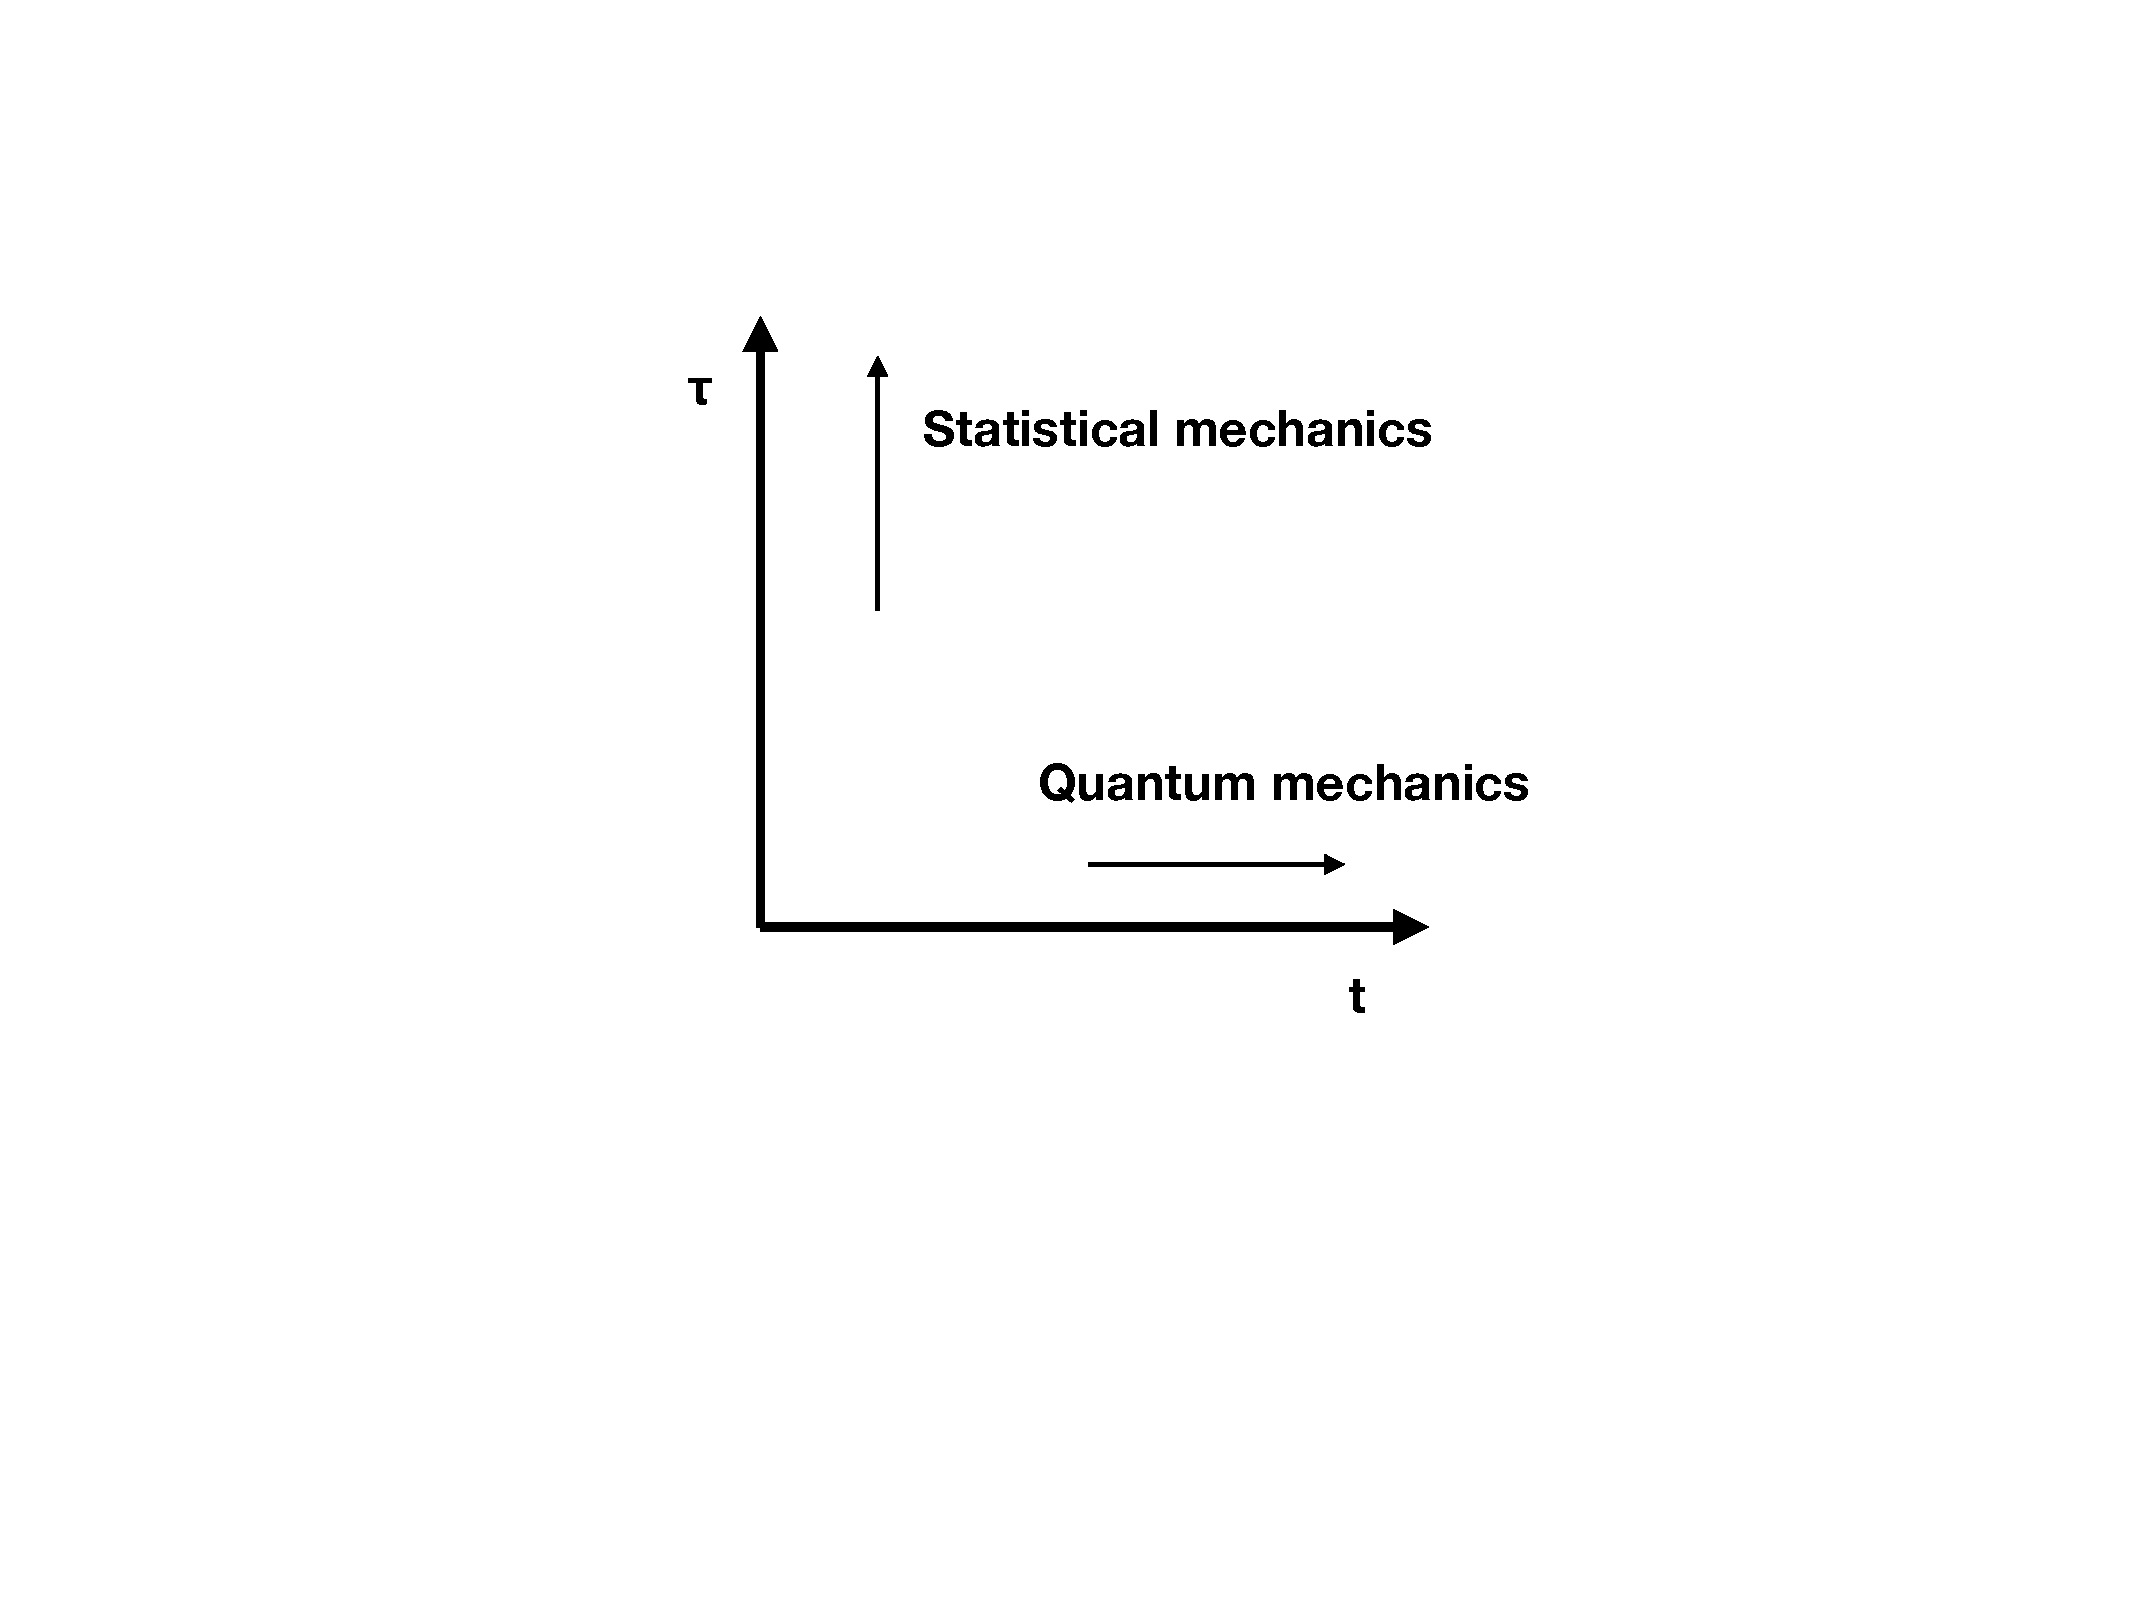
\includegraphics[width=0.8\linewidth]{smech_vs_qmech.pdf}
    \caption{As described in the text, a statistical mechanics problem is equivalent to a Wick rotation applied to a quantum field theory problem. If a single theory of some field is described in the complex time plane, behavior attributed to quantum effects can be imagined as a dependence on the position along the real axis, while statistical behvaior can be thought of as behavior dependent on the position along the imaginary axis.}
    \label{fig:complextime}
\end{figure}
This reflects a generic property that quantum mechanics is like statistical physics with one additional dimension (that is conjugate to the Hamiltonian) \cite{radzihovsky17}.
If we think of time as something living in the complex plane, this implies that the real axis somehow describes quantum mechanical effects, while the imaginary axis $90^{\circ}$ away somehow describes statistical mechanics effects, as seen in Fig.~\ref{fig:complextime}.
While it is interesting to wonder where there is some deep reason for this mathematical quirk, this is neither the time nor place to answer that.

\section{\label{sec:phi4theory}Effective potential in $\phi^4$ theory}
The Lagrangian for $\phi^4$ theory is defined in Eq.~\ref{eq:phi4lagr}.
Based on the effective Hamiltonian we saw in the previous section, we can deduce that this model in particular lives in the $O(1)$ universality class (the Ising model) since $\phi_c$ is real, with this instance in $d=4$ dimensions.

In a typical Landau theory, the parameter $\mu^2$ is related to the temperature, which is generally a tunable parameter in experiment.
As the temperature is changed, the shape of the potential energy term in the Hamiltonian changes until a qualitative difference arises, referred to a phase transition.
In the $4-d$ Ising model we should expect a Wilson Fischer fixed point to separate the ordered and disordered phases, but as previously advertised, no temperature dependence is immediately present in this model.
If we try to compute the effective potential using these new finite temperature rules, it turns out that interactions will introduce the crucially important temperature dependencies \cite{cw73,quiros99}.
\begin{figure}[h]
    \begin{tikzpicture}[baseline=(current bounding box.center)]
        \begin{feynman}
            \vertex (a) at (0,0);
            \vertex (b) at (0.8,0);
            \vertex (e1) at (-0.34641, -0.20);
            \vertex (e2) at (-0.34641, 0.20);
            \diagram*{
                (a)  -- [dashed, half right]      (b),
                (b)  -- [dashed, half right]      (a),
                (e1) -- [dashed, out=30,  in=210] (a),
                (e2) -- [dashed, out=330, in=150] (a)
            };
        \end{feynman}
    \end{tikzpicture}
    \,\,+\,\,
    \begin{tikzpicture}[baseline=(current bounding box.center)]
        \begin{feynman}
            \vertex (a)  at (-0.4, 0);
            \vertex (b)  at (0.4, 0);
            \vertex (e1) at (-0.74641016, -0.20);
            \vertex (e2) at (-0.74641016, 0.20);
            \vertex (e3) at (0.74641016, 0.20);
            \vertex (e4) at (0.74641016, -0.20);
            \diagram*{
                (a)  -- [dashed, half right]      (b),
                (b)  -- [dashed, half right]      (a),
                (e1) -- [dashed, out=30,  in=210] (a),
                (e2) -- [dashed, out=330, in=150] (a),
                (e3) -- [dashed, out=210, in=30]  (b),
                (e4) -- [dashed, out=150, in=330] (b),
            };  
        \end{feynman}
    \end{tikzpicture}
    \,\,+\,\,
    \begin{tikzpicture}[baseline=(current bounding box.center)]
        \begin{feynman}
            \vertex (a)  at (-0.4, 0);
            \vertex (b)  at (0.20, 0.34641);
            \vertex (c)  at (0.20, -0.34641);
            \vertex (e1) at (-0.8, 0.20);
            \vertex (e2) at (-0.8, -0.20);
            \vertex (e3) at (0.20, 0.74641016);
            \vertex (e4) at (0.54641, 0.54641);
            \vertex (e5) at (0.54641, -0.54641);
            \vertex (e6) at (0.20, -0.74641016);
            \diagram*{
                (a)  -- [dashed, out=90,  in=150] (b),
                (b)  -- [dashed, out=330, in=30]  (c),
                (c)  -- [dashed, out=210, in=270] (a),
                (e1) -- [dashed, out=330, in=150] (a),
                (e2) -- [dashed, out=30,  in=210] (a),
                (e3) -- [dashed, out=270, in=90]  (b),
                (e4) -- [dashed, out=210, in=30]  (b),
                (e5) -- [dashed, out=150, in=330] (c),
                (e6) -- [dashed, out=90,  in=270] (c)
            };  
        \end{feynman}
    \end{tikzpicture}
    \,\,+\,\,
    \begin{tikzpicture}[baseline=(current bounding box.center)]
        \begin{feynman}
            \vertex (a)  at (-0.4, 0);
            \vertex (b)  at (0, 0.4);
            \vertex (c)  at (0.4, 0);
            \vertex (d)  at (0, -0.4);
            \vertex (e1) at (-0.74641016, -0.20);
            \vertex (e2) at (-0.74641016, 0.20);
            \vertex (e3) at (-0.20, 0.74641016);
            \vertex (e4) at (0.20, 0.74641016);
            \vertex (e5) at (0.74641016, 0.20);
            \vertex (e6) at (0.74641016, -0.20);
            \vertex (e7) at (0.20, -0.74641016);
            \vertex (e8) at (-0.20, -0.74641016);
            \diagram*{
                (a)  -- [dashed, out=90, in=180]  (b),
                (b)  -- [dashed, out=0,  in=90]   (c),
                (c)  -- [dashed, out=270, in=0]   (d),
                (d)  -- [dashed, out=180, in=270] (a),
                (e1) -- [dashed, out=30,  in=210] (a),
                (e2) -- [dashed, out=330, in=150] (a),
                (e3) -- [dashed, out=300, in=120] (b),
                (e4) -- [dashed, out=240, in=60]  (b),
                (e5) -- [dashed, out=210, in=30]  (c),
                (e6) -- [dashed, out=150, in=330] (c),
                (e7) -- [dashed, out=120, in=300] (d),
                (e8) -- [dashed, out=60,  in=240] (d)
            };  
        \end{feynman}
    \end{tikzpicture}
    \,\,+\,\,...
    \caption{All Feynman diagrams with one $\phi$ loop and external $\phi$ fields are shown. At finite temperature, such diagrams can be interpreted as thermal fluctuations in the $\phi$ field which must be included in calculating the effective potential. Vertices receive a factor of $v/4!$, external lines provide a factor of $\phi_c$, and internal lines add the propagator $-i/(k^2-\mu^2)$. These diagrams can be added analytically in a thermal resummation procedure.}
    \label{fig:selfloops}
\end{figure}

To illustrate this procedure, the effective potential is calculated to one-loop order.
The relevant diagrams can be seen in Fig. \ref{fig:selfloops}.
In this theory, each vertex receives a factor of $\frac{-v}{4!}$.
Furthermore, the symmetry factor for the $n^\text{th}$ diagram $(n>2)$ can be written $S_n = \frac{(2S_1)^n}{2^{n+1}n}$ where $S_1=\frac{4!}{2}$ is the symmetry factor of the first diagram.
This is because there are $n$ external leg pairs connecting to the loop via $\phi^4$ vertices, and there are $2n$ rotations \& reflections of the $n^\text{th}$ diagram (under which Wick's theorem does not provide new field contractions) \cite{quiros99}.

In general, the amplitude of the $n^\text{th}$ diagram is
\begin{equation}
    \V_n^{(1)}(\phi_c) = \int i\frac{d^4k}{(2\pi)^4} \frac{1}{2n} \left(\frac{v\phi_c^2/2}{k^2-\mu^2(\phi)+i\epsilon}\right)^n
\end{equation}
so the one-loop contribution to the effective potential is
\begin{equation}
    \V^{(1)}(\phi_c) = \sum_{n=1}^\infty \V_n^{(1)} = -\frac{i}{2} \int \frac{d^4k}{(2\pi)^4} \ln \left[1- \frac{v\phi_c^2/2}{k^2-\mu^2(\phi)}\right].
\end{equation}
At finite temperature, we apply the thermal field theory prescription for a bosonic field. First we must Wick rotate $k^0\rightarrow ik_E^0$, which removes the factor of $i$ and alters signs in the logarithm
\begin{equation}
    \V^{(1)}(\phi_c) = -\frac{1}{2} \int \frac{d^4k}{(2\pi)^4} \ln \left[1+ \frac{v\phi_c^2/2}{k^2+\mu^2(\phi)}\right].
\end{equation}
Replacing the $dk^0_E$ integral by a sum then dictates
\begin{widetext}
\begin{equation}
    \V^{(1)}(\phi_c, T) = -\frac{T}{2} \int \frac{d^3k}{(2\pi)^3} \sum_{n=-\infty}^{\infty} \ln \left[1+ \frac{v\phi_c^2/2}{k_ik^i+(2\pi T n)^2 + \mu^2(\phi)}\right].
\end{equation}
If we separate the logarithm to remove the $\phi_c$-independent term, we arrive at the generic result \cite{sher89}
\begin{equation}
    \V^{(1)}(\phi_c, T) = \frac{T}{2} \int \frac{d^3k}{(2\pi)^3} \sum_{n=-\infty}^{\infty} \ln \left(k_ik^i+(2\pi T n)^2 + m^2(\phi_c)\right) + \text{Const}.
\end{equation}
\end{widetext}
with $m^2(\phi_c) = \mu^2+v\phi_c^2/2$ the field-dependent mass term.
The integral now looks a bit unwieldy to evaluate, but can be evaluated as done by Dolan \& Jackiw \cite{dj74}: first consider the integrand function and its derivative
\begin{align}
    &f(E) = \sum_{n=-\infty}^{\infty} \ln \left(E^2 + 4\pi^2T^2n^2\right) \\
    &f'(E) = \sum_{n=-\infty}^{\infty} \frac{2E}{E^2 + 4\pi^2T^2n^2}.
\end{align}
where we define $E^2 \equiv k_ik^i + m^2$.
The sum in $f(E)$ clearly diverges, but equipped with the identity
\begin{align}
    \sum_{n=1}^{\infty} \frac{x}{x^2+a^2n^2} &= \frac{1}{a}\sum_{n=1}^{\infty}\frac{x/a}{(x/a)^2+n^2} \\
    &= -\frac{1}{2x} + \frac{\pi}{2a}\coth\left(\frac{\pi x}{a}\right)
\end{align}
we can write the derivative as
\begin{align}
    f'(E) &= 2\left[\frac{1}{E} - \frac{2}{2E} + \frac{2\pi}{4\pi T} \coth\left(\frac{\pi E}{2\pi T}\right)\right] \\
    &= \beta \coth \left(\beta E/2\right) \\
    &= 2\beta \left[\frac{1}{2} + \frac{1}{e^{\beta E}-1}\right]
\end{align}
which is now in an integrable form:
\begin{equation}
    f(E) = 2\beta \left[\frac{E}{2} + \frac{1}{\beta}\ln \left(1-e^{-\beta E}\right)\right] + \text{Const}.
\end{equation}
The constant is presumably infinite, but will be independent of the field $\phi_c$ so we can attribute it to the zero-point energy and drop it. Returning to the effective potential above, we can now evaluate it, dropping the $\phi_c$-independent term as another infinite constant:
\begin{align}
    &\V^{(1)}(\phi_c, T) = \int \frac{d^3k}{(2\pi)^3} \left[\frac{E}{2} + T\ln \left(1-e^{-\beta E}\right)\right] \label{eq:1}
    \\
    &= \frac{T}{2\pi^2} \int_{0}^{\infty} k^2 dk \ln \left(1-e^{-(\beta^2 k^2 + \beta^2 m^2)^{1/2}}\right) \\
    &= \frac{T^4}{2\pi^2} \int_{0}^{\infty} x^2 dx \ln \left(1-e^{-(x^2 + \beta^2m^2)^{1/2}}\right) \\
    &= \frac{T^4}{2\pi^2} J_B(m^2/T^2)
\end{align}
where $J_B$ is the thermal function for bosons
\begin{equation}
    J_B(x^2) = \int_{0}^{\infty} t^2dt\ln \left(1-e^{-\sqrt{t^2+x^2}}\right).
\end{equation}
It conveniently admits a high-temperature series for $x\ll 1$ \cite{quiros99}:
\begin{equation}
\begin{split}
    J_B(x^2) &\underrel{x\ll 1}{\rightarrow} -\frac{\pi^4}{45} +\frac{\pi^2}{12} x^2 - \frac{\pi}{6} x^{3/2} - \frac{1}{32} x^4\ln \frac{x^2}{c_B} \\
    &- 2\pi^{7/2} \sum_{n=1}^\infty (-1)^n \frac{\zeta(2n+1)}{(n+1)!}\Gamma\left(n+\frac{1}{2}\right)\left(\frac{x^2}{4\pi^2}\right)^{n+2}
\end{split}
\end{equation}
with $\ln c_B \equiv 3/2-2\gamma + 4\ln 2\pi \approx 5.41$.
$J_B$ is a well-defined function and contains all of the temperature- and field-dependence in the effective potential, and (as we will see) appears for each boson acquiring a mass from the condensate.
Along with the fermionic partner function $J_F$ (see Sec~\ref{sec:fermions}), it can be seen in Fig.~\ref{fig:thermalfuncs}.
\begin{figure}
    \centering
    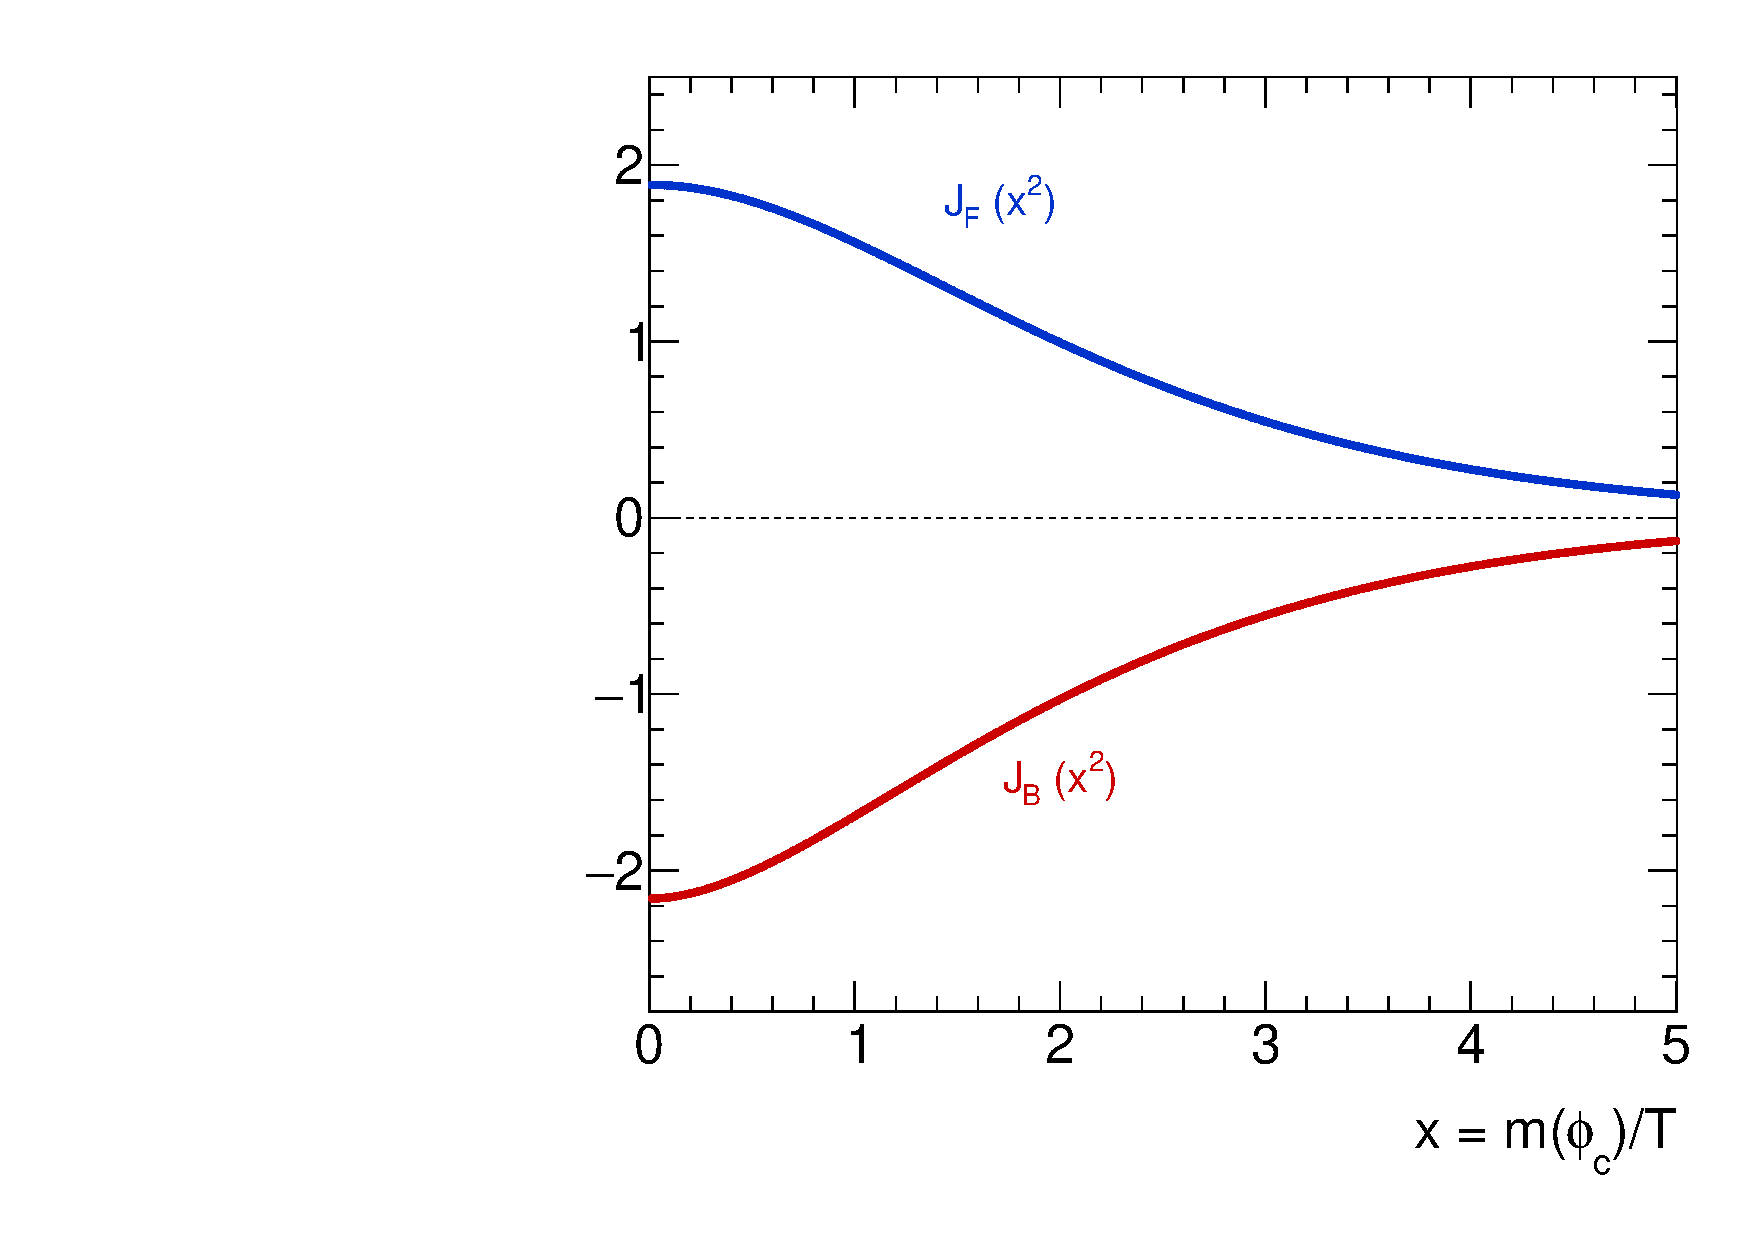
\includegraphics[width=\linewidth]{thermalfuncs.pdf}
    \caption{Both thermal integral functions $J_B$ and $J_F$ are plotted as a function of $m(\phi_c)/T$. At high temperature, these functions admit series expansions which allow the symmetry restoring phase transition to be analyzed.}
    \label{fig:thermalfuncs}
\end{figure}

Repeating the calculation at zero temperature to recover the purely quantum mechanical corrections would yield solely the first term in Eq.~\ref{eq:1} (plus possibly some constant).
The second term therefore describes how thermal fluctuations affect the potential to one loop order.
This term can be expanded for high temperatures (small $\beta$):
\begin{equation}
\begin{split}
    &\approx \frac{T^4}{2\pi^2} \int x^2 dx \left[\ln\left(1-e^{-x}\right) + \frac{\beta^2m^2}{2x}\frac{1}{e^x-1} + \BigO(\beta^4)\right] \\
    &= -\frac{T^4}{6\pi^2}\Gamma(4)\zeta(4) + \frac{m^2 T^2}{4\pi^2} \Gamma(2)\zeta(2) - \frac{1}{12\pi} m^3 T + \BigO(T^{-2}) \\
    &= -\frac{\pi^2}{90}T^4 + \frac{m^2}{24}T^2 - \frac{m^3}{12\pi} T + \BigO(T^{-2}).
\end{split}
\end{equation}
Finally, we reinsert $m^2$ to find the high temperature one-loop effective potential: 
\begin{equation}
    \V^{(1)}(\phi_c, T) = - \frac{\pi^2}{90}T^4 + \frac{\mu^2}{24}T^2 + \frac{v}{48}T^2 \phi_c^2 + h.o.
\end{equation}
where we have dropped the $\propto m^3 T$ term.
(With additional fields present, this term can allow $\phi_c^3$ terms to show up in the effective potential.)
This implies that the finite temperature quadratic term is modified for the condensate \cite{linde05}:
\begin{equation}
    \delta\V (\phi_c, T) = \frac{1}{2}\left(\mu^2 + \frac{v}{24}T^2\right) \phi_c^2.
\end{equation}

We see that thermal fluctuations have a demonstrable effect on the effective potential at nonzero temperature, and can aid our development of a Landau theory around the condensate $\phi_c$.
Working at high temperatures, the theory predicts that the potential will be dominated by a quadratic well around $\phi_c = 0$, so the condensate will disappear.
An intrinsic critical temperature of $T_c \sim \sqrt{\frac{24|\mu^2|}{v}}$ is predicted, below which the quadratic coefficient goes negative and the quartic term becomes non-negligible \cite{linde05}.
If we assume the free parameters have similar values as the standard model Higgs, we get $\mu^2 \sim -100^2~\GeV^2$, $v \sim 4!\lambda \sim 2.88$ so $T_c \sim 300~\GeV \sim 3 \times 10^{15} \text{K}$.
There is no cubic interaction term (without additional fields no cubic term can be acquired) so the phase transition is purely second order.
One caveat of this simplified model is that we could actually go ahead and start calculating critical exponents.
For example, in the Ising model the mean field exponent $\beta$ is given by $M \propto \left|T-T_c\right|^\beta$ with $\beta=\frac{1}{2}$.
In this particular theory we see that, because the phase transition is not present at tree level,
$\phi_c \propto \sqrt{\left(T-T_c\right)^2}$ so we would predict $\beta=1$.
The expectation value $\left<\phi_c\right>$ as a function of temperature can be seen in Fig.~\ref{fig:expectval}; because it is continuous, the phase transition in this theory is not second order (i.e. there is no associated latent heat).
\begin{figure}
    \centering
    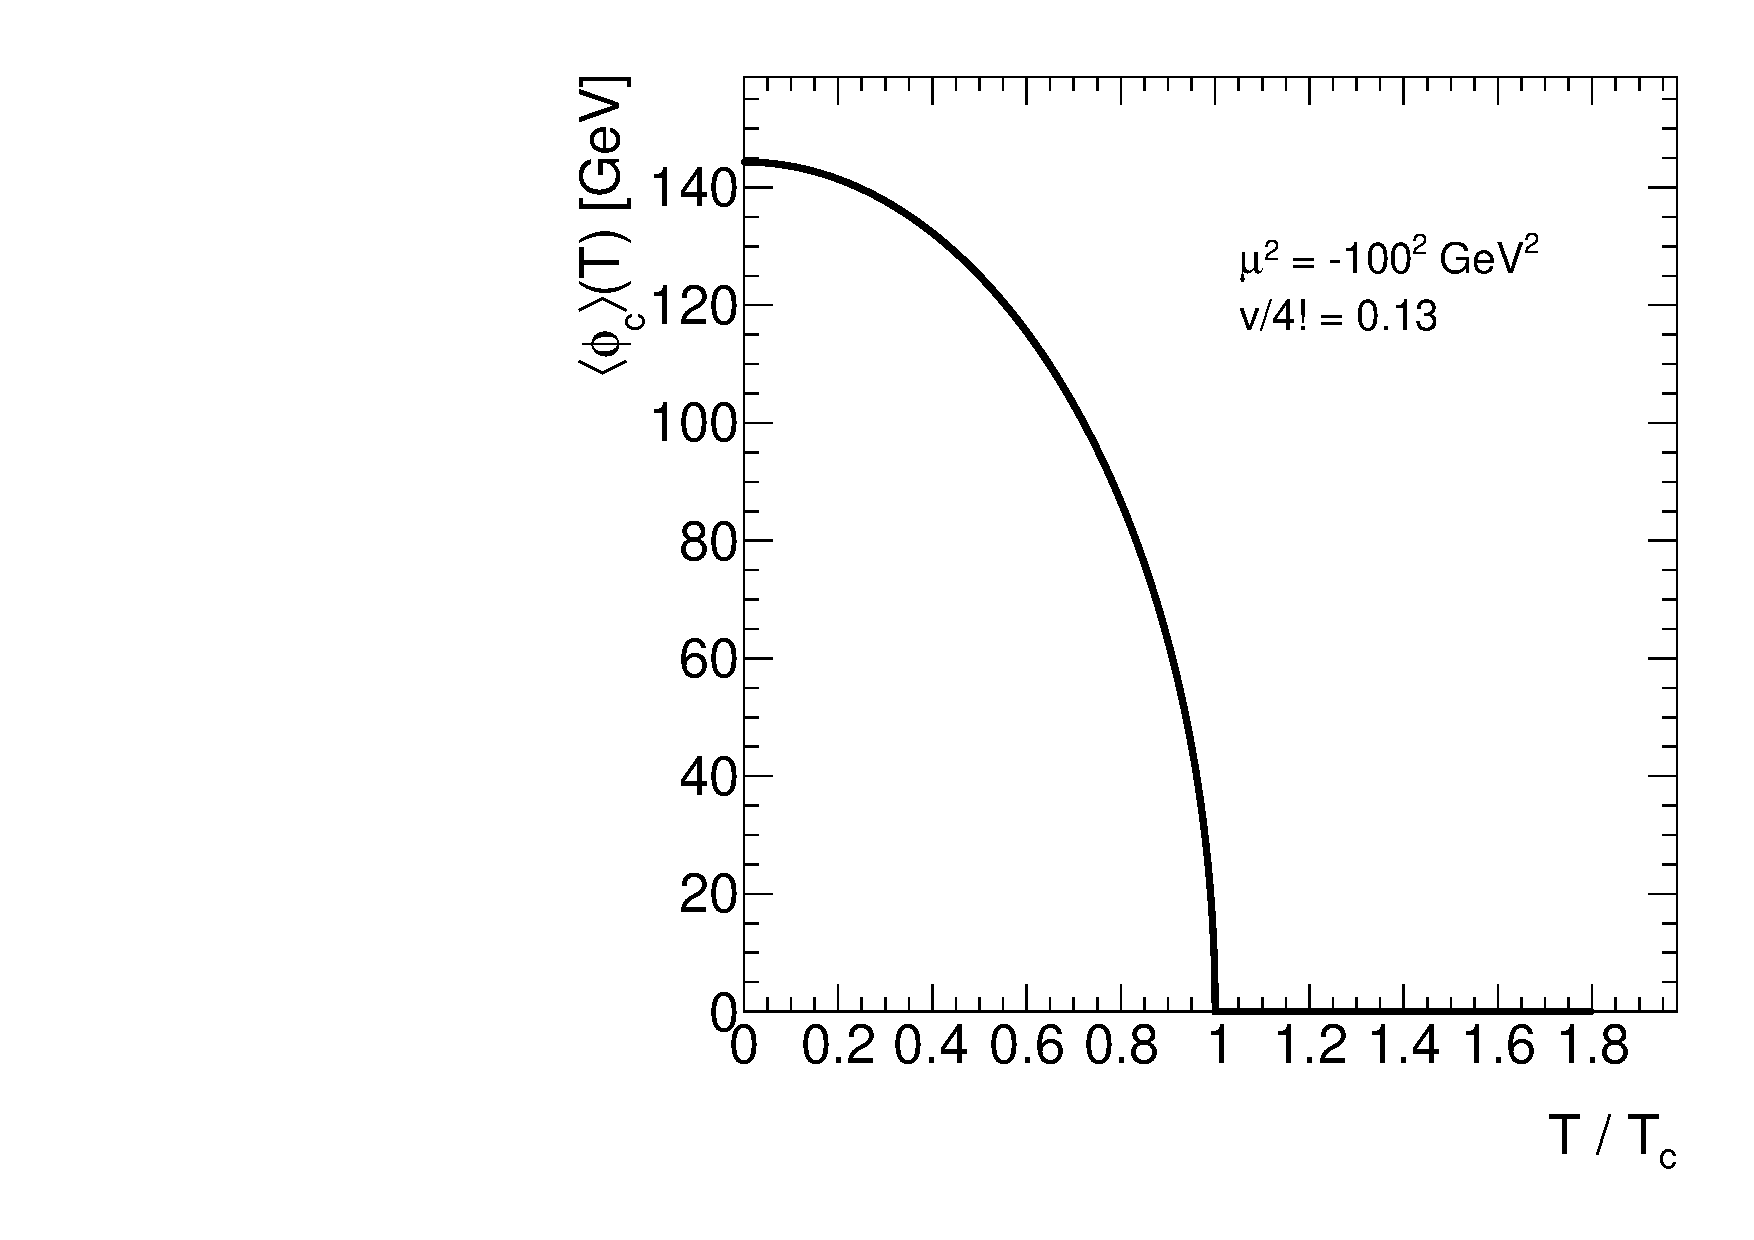
\includegraphics[width=\linewidth]{scalarFieldExpectationValue.pdf}
    \caption{The expected value of $\phi_c$ calculated in the $\phi^4$ mean field theory is plotted as a function of the temperature around $T_c$. At $T_c$, $\phi_c$ is continuous, so the symmetry breaking phase transition is second order.}
    \label{fig:expectval}
\end{figure}

We can also extract the correlation length from the mass term when the system is in the disordered (high temperature) state.
The propagator takes the form
\begin{equation}
    \left<\phi_c \phi_c\right>_\beta \propto \frac{1}{k^2 + \mu^2+\frac{v}{24}T^2}
\end{equation}
so $\xi^{-1}(T) \sim \sqrt{\mu^2+\frac{v}{24}T^2}$.
As $T \rightarrow T_c^+$, this implies $\xi^{-1} \sim \left(T-T_c\right)^{1}$, i.e. $\nu \sim 1$.
For example, at $T=200~\GeV$, the correlation length is predicted to be $\xi \sim \BigO(10^{-3}~\text{fm})$.

\section{\label{sec:bosons}Adding a gauge field}
The minimal extension to this model is to $\phi$ to a gauge field $A_\mu$ with $U(1)$ symmetry group \cite{sher89}.
Generalizations to other symmetry groups is trivial -- since $\phi_c$ will always be in the singlet representation, only the mass and number of degrees of freedom of the gauge bosons can affect the diagram amplitudes.
To maintain gauge invariance, $\phi$ must be promoted to a complex-valued field.
Although, we can still take $\phi_c$ to be real-valued, since gauge invariance will be spontaneously broken in the ordered state anyways\footnote{To see this, write $\phi = \chi_1 + i\chi_2 + \phi_c$, where $\left<\chi_1\right>=\left<\chi_2\right>=0$.}.
The Lagrangian describing this model is identified as scalar electrodynamics:
\begin{align}
    &\Lagr = -\frac{1}{4}F^{\mu\nu}F_{\mu\nu} + \frac{1}{2}(D^\mu\phi)^*D_\mu\phi - \frac{1}{2}\mu^2\phi^2-\frac{v}{4!}\phi^4 \\
    &D_\mu\phi = (\del_\mu - ieA_\mu)\phi
\end{align}
When we introduce a (real-valued) condensate $\phi_c$, the gauge boson picks up a mass as a function $\phi_c$:
\begin{equation}
    \frac{1}{2}(D^\mu\phi_c)^*D_\mu\phi_c \rightarrow 
    \frac{1}{2}e^2\phi_c^2 A^\mu A_\mu
\end{equation}
In order to understand this model at finite temperature, we need to consider the effective potential $\V$ again.
The diagrams in Fig.~\ref{fig:selfloops} still contribute to the one-loop effective potential $\V^{(1)}$, but now the condensate can also interact via the virtual excitations of the gauge boson, as shown in Fig.~\ref{fig:bosonloops}.
\begin{figure}
    \begin{tikzpicture}[baseline=(current bounding box.center)]
        \begin{feynman}
            \vertex (a)  at (0,0);
            \vertex (b)  at (0.8,0);
            \vertex (e1) at (-0.34641, -0.20);
            \vertex (e2) at (-0.34641, 0.20);
            \diagram*{
                (a)  -- [boson, half right]       (b),
                (b)  -- [boson, half right]       (a),
                (e1) -- [dashed, out=30,  in=210] (a),
                (e2) -- [dashed, out=330, in=150] (a)
            };
        \end{feynman}
    \end{tikzpicture}
    \,\,+\,\,
    \begin{tikzpicture}[baseline=(current bounding box.center)]
        \begin{feynman}
            \vertex (a)  at (-0.4, 0);
            \vertex (b)  at (0.4, 0);
            \vertex (e1) at (-0.74641016, -0.20);
            \vertex (e2) at (-0.74641016, 0.20);
            \vertex (e3) at (0.74641016, 0.20);
            \vertex (e4) at (0.74641016, -0.20);
            \diagram*{
                (a)  -- [boson, half right]       (b),
                (b)  -- [boson, half right]       (a),
                (e1) -- [dashed, out=30,  in=210] (a),
                (e2) -- [dashed, out=330, in=150] (a),
                (e3) -- [dashed, out=210, in=30]  (b),
                (e4) -- [dashed, out=150, in=330] (b),
            };  
        \end{feynman}
    \end{tikzpicture}
    \,\,+\,\,
    \begin{tikzpicture}[baseline=(current bounding box.center)]
        \begin{feynman}
            \vertex (a)  at (-0.4, 0);
            \vertex (b)  at (0.20, 0.34641);
            \vertex (c)  at (0.20, -0.34641);
            \vertex (e1) at (-0.8, 0.20);
            \vertex (e2) at (-0.8, -0.20);
            \vertex (e3) at (0.20, 0.74641016);
            \vertex (e4) at (0.54641, 0.54641);
            \vertex (e5) at (0.54641, -0.54641);
            \vertex (e6) at (0.20, -0.74641016);
            \diagram*{
                (a)  -- [boson, out=90,   in=150] (b),
                (b)  -- [boson, out=330,  in=30]  (c)
                (c)  -- [boson, out=210,  in=270] (a),
                (e1) -- [dashed, out=330, in=150] (a),
                (e2) -- [dashed, out=30,  in=210] (a),
                (e3) -- [dashed, out=270, in=90]  (b),
                (e4) -- [dashed, out=210, in=30]  (b),
                (e5) -- [dashed, out=150, in=330] (c),
                (e6) -- [dashed, out=90,  in=270] (c)
            };  
        \end{feynman}
    \end{tikzpicture}
    \,\,+\,\,
    \begin{tikzpicture}[baseline=(current bounding box.center)]
        \begin{feynman}
            \vertex (a)  at (-0.4, 0);
            \vertex (b)  at (0, 0.4);
            \vertex (c)  at (0.4, 0);
            \vertex (d)  at (0, -0.4);
            \vertex (e1) at (-0.74641016, -0.20);
            \vertex (e2) at (-0.74641016, 0.20);
            \vertex (e3) at (-0.20, 0.74641016);
            \vertex (e4) at (0.20, 0.74641016);
            \vertex (e5) at (0.74641016, 0.20);
            \vertex (e6) at (0.74641016, -0.20);
            \vertex (e7) at (0.20, -0.74641016);
            \vertex (e8) at (-0.20, -0.74641016);
            \diagram*{
                (a)  -- [boson, out=90,   in=180] (b),
                (b)  -- [boson, out=0,    in=90]  (c),
                (c)  -- [boson, out=270,  in=0]   (d),
                (d)  -- [boson, out=180,  in=270] (a),
                (e1) -- [dashed, out=30,  in=210] (a),
                (e2) -- [dashed, out=330, in=150] (a),
                (e3) -- [dashed, out=300, in=120] (b),
                (e4) -- [dashed, out=240, in=60]  (b),
                (e5) -- [dashed, out=210, in=30]  (c),
                (e6) -- [dashed, out=150, in=330] (c),
                (e7) -- [dashed, out=120, in=300] (d),
                (e8) -- [dashed, out=60,  in=240] (d)
            };  
        \end{feynman}
    \end{tikzpicture}
    \,\,+\,\,...
    \caption{At high temperatures, there is sufficient energy for $\phi_c$ to create virtual excitations of the massive gauge fields. All diagrams in which a single gauge boson loop is created by the condensate are shown here. Such interactions provide contributions to the effective potential of $\phi_c$, changing its statistical expectation value.}
    \label{fig:bosonloops}
\end{figure}

Evaluation of these diagrams follows similarly to those before, with the scalar propagator generalized to the gauge boson propagator; e.g. in Landau gauge (see any textbook on quantum field theory) \cite{quiros99}
\begin{equation}
    \Pi^\mu_\nu = \frac{-i}{k^2+i\epsilon} \left(g^\mu_\nu - \frac{k^\mu k_\nu}{k^2}\right).
\end{equation}
One can easily show that $\Pi^\mu_\nu \Pi^\nu_\sigma = \left(\frac{-i}{k^2}\right) \Pi^\mu_\nu$ and $\Pi^\mu_\mu = \frac{3i}{k^2}$, which allows the contraction of multiple propagators in a loop with multiple vertices.
At such vertices, the corresponding Feynman rule is to apply a factor of $ie^2g^\mu_\nu$.
External legs contribute factors of $\phi_c$.
For example, the first diagram (two external legs) has an amplitude
\begin{equation}
\begin{split}
    \V^{(1)}_1 &= \frac{1}{2} \int \frac{d^4k}{(2\pi)^4} g^\mu_\nu \Pi_\mu^\nu ie^2\phi_c^2 \\
    &= \frac{3}{2} \int \frac{d^4k}{(2\pi)^4} \frac{-e^2|\phi_c|^2}{k^2}
\end{split}
\end{equation}
and the $n^\text{th}$ diagram introduces $n$ gauge boson propagators (which effectively introduces $n-1$ powers of $-i/k^2$):
\begin{equation}
    \V^{(1)}_n = \frac{3}{2} \int \frac{d^4k}{(2\pi^4)} \frac{1}{n} \left(\frac{-e^2\phi_c^2}{k^2}\right)^n
\end{equation}
which again resums logarithmically
\begin{align}
    \V^{(1)} &= \frac{3}{2} \int \frac{d^4k}{(2\pi^4)} \ln \left[1 + \frac{e^2\phi_c^2}{k^2}\right] \\
    &= \frac{3}{2} \int \frac{d^4k}{(2\pi^4)} \ln \left(k^2 + e^2 \phi_c^2\right).
\end{align}
We have implicitly dropped the infinite zero-point energy contribution which is independent of $\phi_c$.
This expression can be understood as a generalization of the scalar field, where the mass is now the $A^2$ coupling $e^2\phi_c^2$, and there are 3 degrees of freedom that can be independently excited.

At finite temperature, we impose periodicity in the imaginary time direction and continue to drop constants as a function of temperature:
\begin{equation}
\begin{split}
    \V^{(1)} &= \frac{3T}{2} \int \frac{d^3k}{(2\pi)^3} \sum_{n=-\infty}^{\infty} \ln \left(k_ik^i + (2\pi n T)^2 + e^2|\phi_c|^2\right) \\
    &= 3 \int \frac{d^3k}{(2\pi)^3} \left[\frac{E}{2} + T \ln \left(1-e^{-\beta E}\right)\right] \\
    &= \frac{3T}{2\pi^2} \int_{0}^{\infty} k^2 dk \ln \left(1-e^{-(\beta^2k^2+\beta^2 m^2)^{1/2}} \right) \\
    &= \frac{3T^4}{2\pi^2} \int_{0}^{\infty} x^2 dx \ln \left(1-e^{-(x^2+\beta^2 m^2)^{1/2}} \right) \\
    &= \frac{3T^4}{2\pi^2} J_B (m^2/T^2)
\end{split}
\end{equation}
where now $m^2 \equiv e^2\phi_c^2$ is the effective gauge boson mass, and the 3 comes from its internal degrees of freedom (there are 3 polarizations). 
The result here is powerfully simple which allows us to generalize the calculation to any coupled gauge field trivially.
For example, to calculate the effective potential due to the weak interaction, just take 2 copies of $\V$ with $e^2\phi_c^2\rightarrow m_W^2$ and 1 copy with $e^2\phi_c^2\rightarrow m_Z^2$.

In the high temperature limit, we get a similar result from before:
\begin{equation}
\begin{split}
    \V^{(1)} &\approx -\frac{\pi^2}{30}T^4+\frac{m^2}{8}T^2-\frac{m^3}{4\pi}T \\
    &= -\frac{\pi^2}{30}T^4 + \frac{e^2}{8}T^2\phi_c^2 - \frac{e^3}{4\pi}T \phi_c^3
\end{split}
\end{equation}

The contribution from self-interactions of the $\phi$ field still need to be added, but we immediately see that a $\phi^3$ term has emerged, which means the phase transition has a much richer behavior when a gauge field is present.
Because there are two scalar fields ($\phi$ is complex), there are 2 types of self-interactions (essentially it is an XY model).
Essentially, this just boils down to sending either a $\phi$ or $\phi^*$ particle through the loop, resulting in a factor of $2$ difference from the real-valued theory.
The result is a $\phi^3$ term in the effective potential (where we suppose $\phi_c$ is real):
\begin{equation}
    \V (\phi_c) = \frac{1}{2}\left[\mu^2 + \left(\frac{e^2}{4} + \frac{v}{12}\right)T^2\right]\phi_c^2 - \frac{e^3}{4\pi}T\phi_c^3 + \frac{v}{4!}\phi_c^4.
\end{equation}
This potential allows for either first or second order phase transitions between the disordered and ordered $\phi_c$ states.

The minima are described by
\begin{equation}
\begin{split}
    &\frac{d\V}{d\phi_c} = 0 = \phi_c \left(\mu^2 + \left(\frac{e^2}{4}+\frac{v}{12}\right)T^2 -\frac{3e^3}{4\pi}T\phi_c + \frac{v}{3!}\phi_c^2\right) \\
    &0 = \mu^2 + \left(\frac{e^2}{4}+\frac{v}{12}\right)T^2 -\frac{3e^3}{4\pi}T\phi_c + \frac{v}{3!}\phi_c^2 \\
    &\phi_c = \frac{3}{v}\left[\frac{3e^3}{4\pi}T \pm \sqrt{\frac{9e^6}{16\pi^2}T^2-\frac{4v}{3!}\left(\mu^2+\left(\frac{e^2}{4}+\frac{v}{12}\right)T^2\right)}\right] \\
    &\phi_c = \frac{9e^3}{4\pi v}T \left[1 \pm \sqrt{1 - \frac{32\pi^2 v}{27e^6 T^2}\left(\mu^2 + \left(\frac{e^2}{4}+\frac{v}{12}\right)T^2\right)}\right].
\end{split}
\end{equation}
Since $\phi_c$ is chosen to be a real quantity, there is a particular temperature at which one of the extrema becomes imaginary (and thus is no longer a solution):
\begin{align}
    &\mu^2 + \left(\frac{e^2}{4}+\frac{v}{12}\right)T_c^2 = \frac{27e^6}{32\pi^2 v}T_c^2 \\
    &T_c = \sqrt{\frac{|\mu^2|}{\frac{e^2}{4} + \frac{v}{12} - \frac{27e^6}{32\pi^2 v}}} \label{eq:bosontc}.
\end{align}
At this temperature there are two minima with a free energy barrier between them; this is indicative of a first order phase transition.
However, if the denominator in Eq.~\ref{eq:bosontc} is negative, this temperature doesn't exist, so the phase transition can only be continuous!
This shows that the gauge bosons control whether the phase transition is first order.

\section{\label{sec:fermions}Adding a fermion field}
In QED, Dirac spinors are sufficient to couple electrons to the electromagnetic field.
However due to the weak interaction violating $CP$ symmetry, Weyl spinors are favored in the standard model over Dirac spinors.
This requires the fermion mass terms to go to zero, which contradicts experiment.
The resolution is that in the standard model the Higgs not only provides a mass to the $W$ and $Z$ bosons, but also to the fermions via the Yukawa interaction.
So in our analysis we must also study the effect of coupling $\Phi$ to a fermion $\Psi$ in the Lagrangian. \\

A simple Lagrangian for a model with a $\phi$ field plus one massless fermion $\psi$ is
\begin{equation}
    \Lagr = \Lagr_{GB} + i\bar{\psi}\slashed{D}\psi - h_{\psi} \phi \bar{\psi}\psi
\end{equation}
where $\Lagr_{GB}$ is the $\phi, A_\mu$ Lagrangian from Sec.~\ref{sec:bosons} and $h_{\psi}$ is the dimensionless Yukawa coupling.
After spontaneous symmetry breaking, $\phi \rightarrow \phi_c + \chi$ so the Dirac mass $m_\psi$ is proportional to the condensate value and the $\phi-\psi$ coupling: $m_\psi= h_{\psi} \phi_c$.

\begin{figure}
    \begin{tikzpicture}[baseline=(current bounding box.center)]
        \begin{feynman}
            \vertex (a) at  (-0.35, 0);
            \vertex (b) at  (0, 0.35);
            \vertex (c) at  (0.35, 0);
            \vertex (d) at  (0, -0.35);
            \vertex (e1) at (-0.7, 0);
            \vertex (e2) at (0.7, 0);
            \diagram*{
                (a)  -- [fermion, out=90,  in=180]  (b),
                (b)  -- [         out=0,  in=90]   (c),
                (c)  -- [fermion, out=270,  in=0]  (d),
                (d)  -- [         out=180, in=270] (a),
                (e1) -- [dashed, out=0,   in=180]  (a),
                (e2) -- [dashed, out=180, in=0]    (c),
            };  
        \end{feynman}
    \end{tikzpicture}
    \,\,+\,\,
    \begin{tikzpicture}[baseline=(current bounding box.center)]
        \begin{feynman}
            \vertex (a) at  (-0.4, 0);
            \vertex (b) at  (0, 0.4);
            \vertex (c) at  (0.4, 0);
            \vertex (d) at  (0, -0.4);
            \vertex (e1) at (-0.7, 0);
            \vertex (e2) at (0, 0.7);
            \vertex (e3) at (0.7, 0);
            \vertex (e4) at (0, -0.7);
            \diagram*{
                (a)  -- [fermion, quarter left]   (b),
                (b)  -- [         quarter left]   (c),
                (c)  -- [fermion, quarter left]   (d),
                (d)  -- [         quarter left]   (a),
                (e1) -- [dashed, out=0,   in=180] (a),
                (e2) -- [dashed, out=270, in=90]  (b),
                (e3) -- [dashed, out=180, in=0]   (c),
                (e4) -- [dashed, out=90,  in=270] (d),
            };  
        \end{feynman}
    \end{tikzpicture}
    \,\,+\,\,
    \begin{tikzpicture}[baseline=(current bounding box.center)]
        \begin{feynman}
            \vertex (a) at  (-0.4, 0);
            \vertex (b) at  (-0.2, 0.34641);
            \vertex (c) at  (0.2, 0.34641);
            \vertex (d) at  (0.4, 0);
            \vertex (e) at  (0.2, -0.34641);
            \vertex (f) at  (-0.2, -0.34641);
            \vertex (e1) at (-0.7, 0);
            \vertex (e2) at (-0.35, 0.60622);
            \vertex (e3) at (0.35, 0.60622);
            \vertex (e4) at (0.7, 0);
            \vertex (e5) at (0.35, -0.60622);
            \vertex (e6) at (-0.35, -0.60622);
            \diagram*{
                (a)  -- [fermion, out=90,  in=210] (b),
                (b)  -- [         out=30,  in=150] (c),
                (c)  -- [         out=330, in=90]  (d),
                (d)  -- [fermion, out=270, in=30]  (e),
                (e)  -- [         out=210, in=330] (f),
                (f)  -- [         out=150, in=270] (a),
                (e1) -- [dashed, out=0,    in=180] (a),
                (e2) -- [dashed, out=300,  in=120] (b),
                (e3) -- [dashed, out=240,  in=60]  (c),
                (e4) -- [dashed, out=180,  in=0]   (d),
                (e5) -- [dashed, out=120,  in=300] (e),
                (e6) -- [dashed, out=60,   in=240] (f),
            };  
        \end{feynman}
    \end{tikzpicture}
    \,\,+\,\,
    \begin{tikzpicture}[baseline=(current bounding box.center)]
        \begin{feynman}
            \vertex (a) at  (-0.4, 0);
            \vertex (b) at  (-0.28284, 0.28284);
            \vertex (c) at  (0, 0.4);
            \vertex (d) at  (0.28284, 0.28284);
            \vertex (e) at  (0.4, 0);
            \vertex (f) at  (0.28284, -0.28284);
            \vertex (g) at  (0, -0.4);
            \vertex (h) at  (-0.28284, -0.28284);
            \vertex (e1) at (-0.7, 0);
            \vertex (e2) at (-0.49497, 0.49497);
            \vertex (e3) at (0, 0.7);
            \vertex (e4) at (0.49497, 0.49497);
            \vertex (e5) at (0.7, 0);
            \vertex (e6) at (0.49497, -0.49497);
            \vertex (e7) at (0, -0.7);
            \vertex (e8) at (-0.49497, -0.49497);
            \diagram*{
                (a)  -- [fermion, out=90,  in=225] (b),
                (b)  -- [         out=45,  in=180] (c),
                (c)  -- [         out=0,   in=135] (d),
                (d)  -- [         out=315, in=90]  (e),
                (e)  -- [fermion, out=270, in=45]  (f),
                (f)  -- [         out=225, in=0]   (g),
                (g)  -- [         out=180, in=315] (h),
                (h)  -- [out=135, in=270] (a),
                (e1) -- [dashed, out=0,    in=180] (a),
                (e2) -- [dashed, out=315,  in=135] (b),
                (e3) -- [dashed, out=270,  in=90]  (c),
                (e4) -- [dashed, out=225,  in=45]  (d),
                (e5) -- [dashed, out=180,  in=0]   (e),
                (e6) -- [dashed, out=135,  in=315] (f),
                (e7) -- [dashed, out=90,   in=270] (g),
                (e8) -- [dashed, out=45,   in=225] (h),
            };  
        \end{feynman}
    \end{tikzpicture}
    \,\,+\,\,...
    \caption{The set of Feynman diagrams with all possible condensate interactions occurring via a single fermion loop. Due to each fermion propagator providing a $\gamma^\mu$ matrix, diagrams with an odd number of fermion propagators vanish under the spinor trace. Therefore such diagrams only contribute to the even powers of $\phi_c$ in the effective potential.}
    \label{fig:fermionloops}
\end{figure}
We now calculate the relevant diagrams in the one-loop effective potential.
We proceed as before, calculating all possible Feynman diagrams with exactly one internal fermion loop and all external $\phi_c$ fields.
This series of diagrams is shown in Fig.~\ref{fig:fermionloops}.
The diagram structure is slightly different than before, with only one $\phi_c$ at each vertex, however they still have similar properties.
The Feynman rules for fermions can be found in any quantum field theory text, including instructions on how to evaluate traces of $\gamma$ matrices, so this is not shown here and we will simply quote the results.
Notably however, no diagram with an odd number of internal propagators can exist, as $\Tr \Pi_{k=1}^{2n+1} \gamma^{\mu_k} = 0$ for all integer $n$.
For Dirac fermions (in particular top quarks, which couple the most strongly), the $(2n)^\text{th}$ diagram takes the form \cite{quiros99}
\begin{equation}
    \V^{(1)}_n = -\frac{1}{2n}\int \frac{d^4k}{(2\pi)^4} \frac{m_\psi^2}{k^{2n}} \times 4
\end{equation}
where the 4 comes from the 4 Dirac spinor degrees of freedom and the minus sign for the fermion loop
\footnote{For Weyl spinors, the 4 becomes a 2.}.
Summing over all diagrams yields a similar function from before:
\begin{align}
    \V^{(1)} &= -2i \int \frac{d^4k}{(2\pi)^4} \sum_{n=1}^{\infty} \frac{1}{n}\left(\frac{m_\psi^2}{k^2}\right)^n \\
    &= -2i \int \frac{d^4k}{(2\pi)^4} \ln \left(1-\frac{m_\psi^2}{k^2}\right) \\
    &\underrel{it\rightarrow \tau}{\rightarrow} -2 \int \frac{d^4k}{(2\pi)^4} \left[\ln \left(k^2 + m_\psi^2\right) + \ln k^2 \right]
\end{align}
As usual, the $\ln k^2$ is independent of the condensate so it does not affect the phase transition. At finite temperature, we require the fermion field to be antiperiodic in the imaginary time direction:
\begin{align}
    \V^{(1)} &= -2T \int \frac{d^3k}{(2\pi)^3} \sum_{n=-\infty}^{\infty} \ln \left(k_ik^i+ \left((2n+1)\pi T\right)^2 +m_\psi^2\right).
\end{align}
The fermionic phase shift effectively converts the previous Bose-Einstein function to a Fermi-Dirac one.
This can be seen by directly evaluating the integrand; again using the shorthand $E^2 \equiv k_ik^i + m_\psi^2$ and $a\equiv \pi T$
\begin{equation}
\begin{split}
    f(E) &\equiv \sum_{n=-\infty}^{\infty} \ln \left(E^2 + (2n+1)^2a^2\right) \\
    &= \sum_{n\in \text{odds}} \ln \left(E^2 + (na)^2\right) \\
    &= \sum_{n=-\infty}^{\infty} \ln \left(E^2 + (na)^2\right) - \sum_{n\in \text{evens}} \ln \left(E^2 + (na)^2\right) \\
    &= \sum_{n=-\infty}^{\infty} \left[\ln \left(E^2 + (na)^2\right) - \ln \left(E^2 + (2na)^2\right)\right]
\end{split}
\end{equation}
The sum can be evaluated via summing its derivative from $n=1$ to $\infty$ twice, plus the $n=0$ term:
\begin{equation}
\begin{split}
    f'(E) &= \sum_{n=-\infty}^{\infty} \left(\frac{2E}{E^2+(na)^2}-\frac{2E}{E^2+(2na)^2}\right) \\
    &= \frac{1}{a}\sum_{n=-\infty}^{\infty} \left(\frac{2(E/a)}{(E/a)^2+n^2} - \frac{1}{2} \frac{2(E/2a)}{(E/2a)^2+n^2}\right) \\
    %&= \frac{2}{a}\left[-\frac{a}{E} + \pi \coth\left(\frac{\pi E}{a}\right) + \frac{a}{E} - \right.\\
    %&\left. \frac{1}{2} \left(-\frac{1}{(E/2a)} + \pi \coth \left(\frac{\pi E}{2a}\right) + \frac{1}{E/2a}\right) \right] \\
    &= \frac{2\pi}{a}\coth\left(\frac{\pi E}{a}\right) - \frac{\pi}{a}\coth\left(\frac{\pi E}{2a}\right) \\
    &= \frac{2}{T}\coth\beta E - \frac{1}{T}\coth\left(\beta E/ 2\right) \\
    &= \frac{1}{T}\left(\coth \beta E - \text{csch}\beta E\right) \\
    &= \frac{1}{T}\tanh(\beta E / 2) = \frac{2}{T}\left(\frac{1}{2} - \frac{1}{e^{\beta E} +1}\right)
\end{split}
\end{equation}
which is integrable, so
\begin{equation}
    f(E) = \frac{2}{T} \left[\frac{E}{2} + T \ln \left(1 + e^{-\beta E}\right)\right] + \text{Const.}
\end{equation}
Returning to the fermionic one-loop potential, we find an infinite zero-temperature zero-point-energy term (which we drop) and a Fermi-Dirac-like contribution:
\begin{align}
    \V^{(1)} &= -4 \int \frac{d^3k}{(2\pi)^3} \left[\frac{E}{2} + T\ln \left(1+e^{-\sqrt{\beta^2 k^2+\beta^2m_\psi^2}}\right)\right]\\
    &= -\frac{2T}{\pi^2} \int_{0}^{\infty} k^2 dk \ln \left(1+e^{-\sqrt{\beta^2 k^2+\beta^2m_\psi^2}}\right) \\
    &= -\frac{2T^4}{\pi^2} J_F \left(m_\psi^2/T^2\right)
\end{align}
where the fermion integral function is defined similarly to its bosonic counterpart
\begin{equation}
    J_F \left(x^2\right) \equiv \int_0^\infty t^2 dt \ln \left(1+e^{-\sqrt{t^2+x^2}}\right)
\end{equation}
and admits an expansion at $x \ll 1$ \cite{quiros99}
\begin{equation}
\begin{split}
    J_F \left(x^2\right) &\underrel{x\ll1}{\rightarrow} \frac{7\pi^4}{360} - \frac{\pi^2}{24}x^2 - \frac{1}{32} x^4\ln \frac{x^2}{c_f}
    %&-\frac{\pi^{7/2}}{4}\sum_{n=1}^{\infty} (-1)^n \frac{\zeta(2n+1)}{(n+1)!} \left(1-2^{-2n-1}\right) \Gamma \left(n+\frac{1}{2}\right)\left(\frac{x^2}{\pi^2}\right)^{2n+1}
\end{split}
\end{equation}
where $\ln c_f=3/2 + 2\ln \pi - \gamma \approx 2.64$.
So at high temperatures the one-loop fermion contribution goes as
\begin{equation}
    \V^{(1)} \approx -\frac{7\pi^2}{180}T^4 + \frac{1}{12}m_\psi^2 T^2 + \frac{1}{16\pi^2}m_\psi^4\ln\frac{m_\psi^2}{c_f T^2}.
\end{equation}
Without looking at the combined effective potential, there are some simple comments to make about this result.
Notably, there is no $m^3$ term, unlike for bosons, so we do not expect Yukawa interactions to allow the phase transition to be first order.
In fact, the contribution to the mass and quartic terms are positive, so any cubic interaction term introduced by the gauge fields will be suppressed by fermion loops.
One interpretation of this result is that fermions prefer the phase transition to be continuous.
Naively we might then assume that the particle which most strongly couples to the Higgs should dictate the order of the phase transition.
This is somewhat justified as the contribution from each type of interaction is explicitly dependent on the relevant coupling constant.
Because we observe $m_\text{top} > m_H > m_Z > m_W$, this leads to the simple prediction that the phase transition in electroweak theory is continuous.
To see whether this is indeed the case, we need to use the tools we have developed to evaluate the full effective potential from interactions with all fields.

\section{\label{sec:smphasepred}Standard Model Effective Potential}
The gauge boson sector of the standard model is as defined in Eq.~\ref{eq:smlagr}.
Each fermion is provided with a kinetic term which applies a covariant derivative in the appropriate representation of each gauge group, and gains a mass through the Yukawa couplings after spontaneous symmetry breakdown.
As an approximation, only the particles which have substantial Higgs couplings -- i.e. the largest masses -- are considered here.
All leptonic and all quark contributions to the $\phi_c$ effective potential are ignored, with the exception of the top quark (which has a very large mass).
In this approximation, the effective potential can be calculated at one-loop order, following the instructions for bosons and fermions already outlined.
Contributions for each species can be separately evaluated, or we can just apply the results from each previous section to obtain the general result
\begin{widetext}
\begin{equation}
    \V_\text{thermal}^{(1)} (\phi_c, T) = \frac{T^4}{2\pi^2} \left(\sum_{i\in\text{bosons}}g_i J_B \left(\frac{m_i^2(\phi_c)}{T^2}\right) - \sum_{i\in\text{fermions}}g_i J_F\left(\frac{m_i^2(\phi_c)}{T^2}\right)\right)
\end{equation}
with $g_i$ the number of degrees of freedom for particle $i$.
This is the purely thermal contribution to the effective potential, but as advertised in Sec.~\ref{sec:ftqft}, an additional term from quantum interactions, referred to as the Coleman Weinberg potential must also be added \cite{cw73,quiros99,long12,cmr18}. At one-loop order, this contribution takes the form \cite{cmr18}
\begin{equation}
    \V_\text{CW}^{(1)} (\phi_c) = \frac{1}{64\pi^2}\left(\sum_{i\in\text{bosons}}g_i m_i^4(\phi_c) \left(\ln \frac{m_i^2(\phi_c)}{\Lambda^2} - c_i\right) - \sum_{i\in\text{fermions}}g_i m_i^4(\phi_c) \left(\ln \frac{m_i^2(\phi_c)}{\Lambda^2} - c_i\right)\right)
\end{equation}
with $\Lambda$ the renormalization scale (i.e. the momentum cutoff scale) and $c_i = 3/2$ for scalars and fermions, or $5/2$ for vector bosons.\footnote{The one-loop Coleman Weinberg potential can be derived from the same set of diagrams that we looked at, but using the standard Feynman rules at $T=0$.}
\end{widetext}

For the standard model, the thermally resummed effective potential can then be written in the form \cite{quiros99,ah92}
\begin{equation}
    \V(\phi_c, T) = D\left(T^2-T_0^2\right)\phi_c^2 - ET \phi_c^3 + \frac{\lambda(T)}{4} \phi_c^4
\end{equation}
with some convenient parameters defined as
\begin{align}
    &D = \frac{2m_W^2+m_Z^2 + 2m_\text{top}^2}{8v^2} \approx 0.167 \\
    &E = \frac{2m_W^3 + m_Z^3}{4\pi v^3} \approx 0.00959 \\
    &T_0^2 = \frac{m_h^2-8Bv^2}{4D} \\
    &B = \frac{3}{64\pi^2 v^4} \left(2m_W^4+m_Z^4-4m_\text{top}^4\right) \approx -0.00443 \\
    &\lambda(T) = \lambda - \frac{3}{16\pi^2v^4} \left(2m_W^4 \ln \frac{m_W^2}{C_B T^2} + \right. \nonumber \\
    &\mytab \left. m_Z^4 \ln \frac{m_Z^2}{C_B T^2} - 4 m_\text{top}^4 \ln \frac{m_\text{top}^2}{C_FT^2} \right).
\end{align}
with $\ln C_{B,F} = \ln c_{B,F} - 3/2$. 
This expansion is derived using the provided expansions for $J_{B/F}$ valid at high temperatures, $T\gg m_\text{top}$.
We see immediately that the mass of the top does not affect the cubic term $E$, which is what we previously argued for the general fermion case.
Only the W and Z bosons affect the cubic term, which means that they control the order of the phase transition. 
Because all of these particles gain their mass from the Higgs' mechanism, each mass is related to $\phi_c$ \cite{pdg2018}:
\begin{align}
    &m_h^2 = 3\lambda \phi_c^2 - \lambda v^2 \approx 125.2~\GeV \\
    &m_W^2 = \frac{g^2}{4}\phi_c^2 \approx 80.4~\GeV \\
    &m_Z^2 = \frac{g^2+g'^2}{4}\phi_c^2 \approx 91.2~\GeV \\
    &m_\text{top}^2 = \frac{h_\text{top}^2}{2}\phi_c^2 \approx 173.0~\GeV.
\end{align}

Furthermore, $\phi_c$ itself has been measured at $T\rightarrow0$ since it is related to the low-energy vector-minus-axial coupling $G_F$: $v \approx 246~\GeV$, although in this paper it is more useful to say $v=246~\GeV$ since the value of $\phi_c$ can change depending on the phase of the system.

On their own, these parameters provide useful insight to the physics of the phase transition.
For example, setting $m_Z = m_W = 0$ briefly, we see that the mass term of $\phi_c$ becomes negative for temperatures $T < T_0$, so the critical temperature of the phase transition must be $T_0$.

We can also follow the procedure of Sec.~\ref{sec:phi4theory} and extract the correlation length in the disordered phase.
At that point, the only relevant term is the quadratic interation so the correlation length must be given by
\begin{equation}
    \xi^{-1}(T) \sim \sqrt{D(T^2-T_0^2)} 
\end{equation}
and therefore $\nu \sim 1$ in the full standard model.
This is not unexpected, since the additional fields do not change the structure of the quadratic term, although the constants $D$ and $T_0$ depend on what fields couple to $\phi_c$.

For the general case, we can minimize the effective free energy by the usual procedure. All derivative terms are positive definite, so they are minimized at $0$.
At high temperatures, the quadratic term in $\phi_c$ dominates so the only extrema is the global minimum at $\phi_c = 0$.
As the temperature is lowered, the cubic and quadratic terms contribute more, so we need to minimize the effective potential with respect to $\phi_c$:
\begin{align}
    &\frac{d\V}{d\phi_c} = 0 = \phi_c\left[2D\left(T^2-T_0^2\right) - 3ET\phi_c + \lambda(T)\phi_c^2\right] \\
    &2D\left(T^2-T_0^2\right) - 3ET\phi_c + \lambda(T)\phi_c^2 = 0 \\
    &\phi_c = \frac{3ET}{2\lambda(T)}\left(1 \pm \sqrt{1-\frac{8D(T^2-T_0^2)\lambda(T)}{9E^2T^2}}\right)\label{eq:2}.
\end{align}
\begin{widetext}
We can actually arrange these extrema in increasing order:
\begin{equation}
    0 < \frac{3ET}{2\lambda(T)}\left(1 - \sqrt{1-\frac{8D(T^2-T_0^2)\lambda(T)}{9E^2T^2}}\right) < \frac{3ET}{2\lambda(T)}\left(1 + \sqrt{1-\frac{8D(T^2-T_0^2)\lambda(T)}{9E^2T^2}}\right).
\end{equation}
Thus we conclude that the minima must be the smallest and largest, with the maximum in the middle.
\end{widetext}

From extremizing the radicand, there is a critical temperature which emerges, usually referred to as $T_1$.
It is defined such that
\begin{equation}
\begin{split}
    &\frac{8D(T_1^2-T_0^2)\lambda(T_1)}{9E^2T^2} = 1 \\
    &T_1^2 = \frac{8DT_0^2\lambda(T_1)}{8D\lambda(T_1)-9E^2}.
\end{split}
\end{equation}
At this temperature, the nontrivial minimum is taken from \ref{eq:2}:
\begin{equation}
    \phi_c = \frac{3ET_1}{2\lambda(T_1)} \neq 0.
\end{equation}
Essentially, $T_1$ defines the temperature at which the maximum and $\phi_c \neq 0$ minimum coincide; at temperatures $T>T_1$, the radicand is imaginary so the only solution occurs at $\phi_c = 0$ and symmetry is restored.
If $T<T_1$, an additional local minimum exists, so it is in this region that the symmetric and asymmetric states can coexist.

A second critical temperature corresponds to when the extremum at $\phi_c = 0$ coincides with the maximum; at temperatures below this, $\phi_c = 0$ will be a maxmimum and therefore the condensate will move towards one of the minima\footnote{In the jargon of condensed matter physics, this temperature is interpreted as the spinoidal point.}.
The temperature for this to occur is defined by $0 = 8D\left(T^2-T_0^2\right)\lambda(T)$, i.e.
\begin{equation}
    T = T_0.
\end{equation}
In the regime $T_0 < T < T_1$, there are two minima so both the symmetric and asymmetric phases coexist.

Although not fully justified, a reasonable starting point for understanding conditions on the phase transition being first order is to first approximate $\lambda(T) \approx \lambda$ \cite{long12}.
$\lambda(T)$ only varies with temperature logarithmically, so as long as temperature does not vary by orders of magnitude $\lambda'(T) \sim 0$.
With this assumption, we can approximate the critical temperatures to help search of a first order phase transition.
For example, \cite{dine92} examines a model with $m_h=50~\GeV$ and $m_\text{top}=120~\GeV$ \footnote{Note that neither of these particles had yet been discovered at the time of publication, although these values make illustration of the first order transition simpler.}.
The critical temperatures for the transition can then be approximated as $T_0 \sim 84~\GeV$ and $T_1 \sim 86~\GeV$.
In Fig.~\ref{fig:fopt}, the potential is plotted for a variety of temperatures in this region.
\begin{figure}
    \centering
    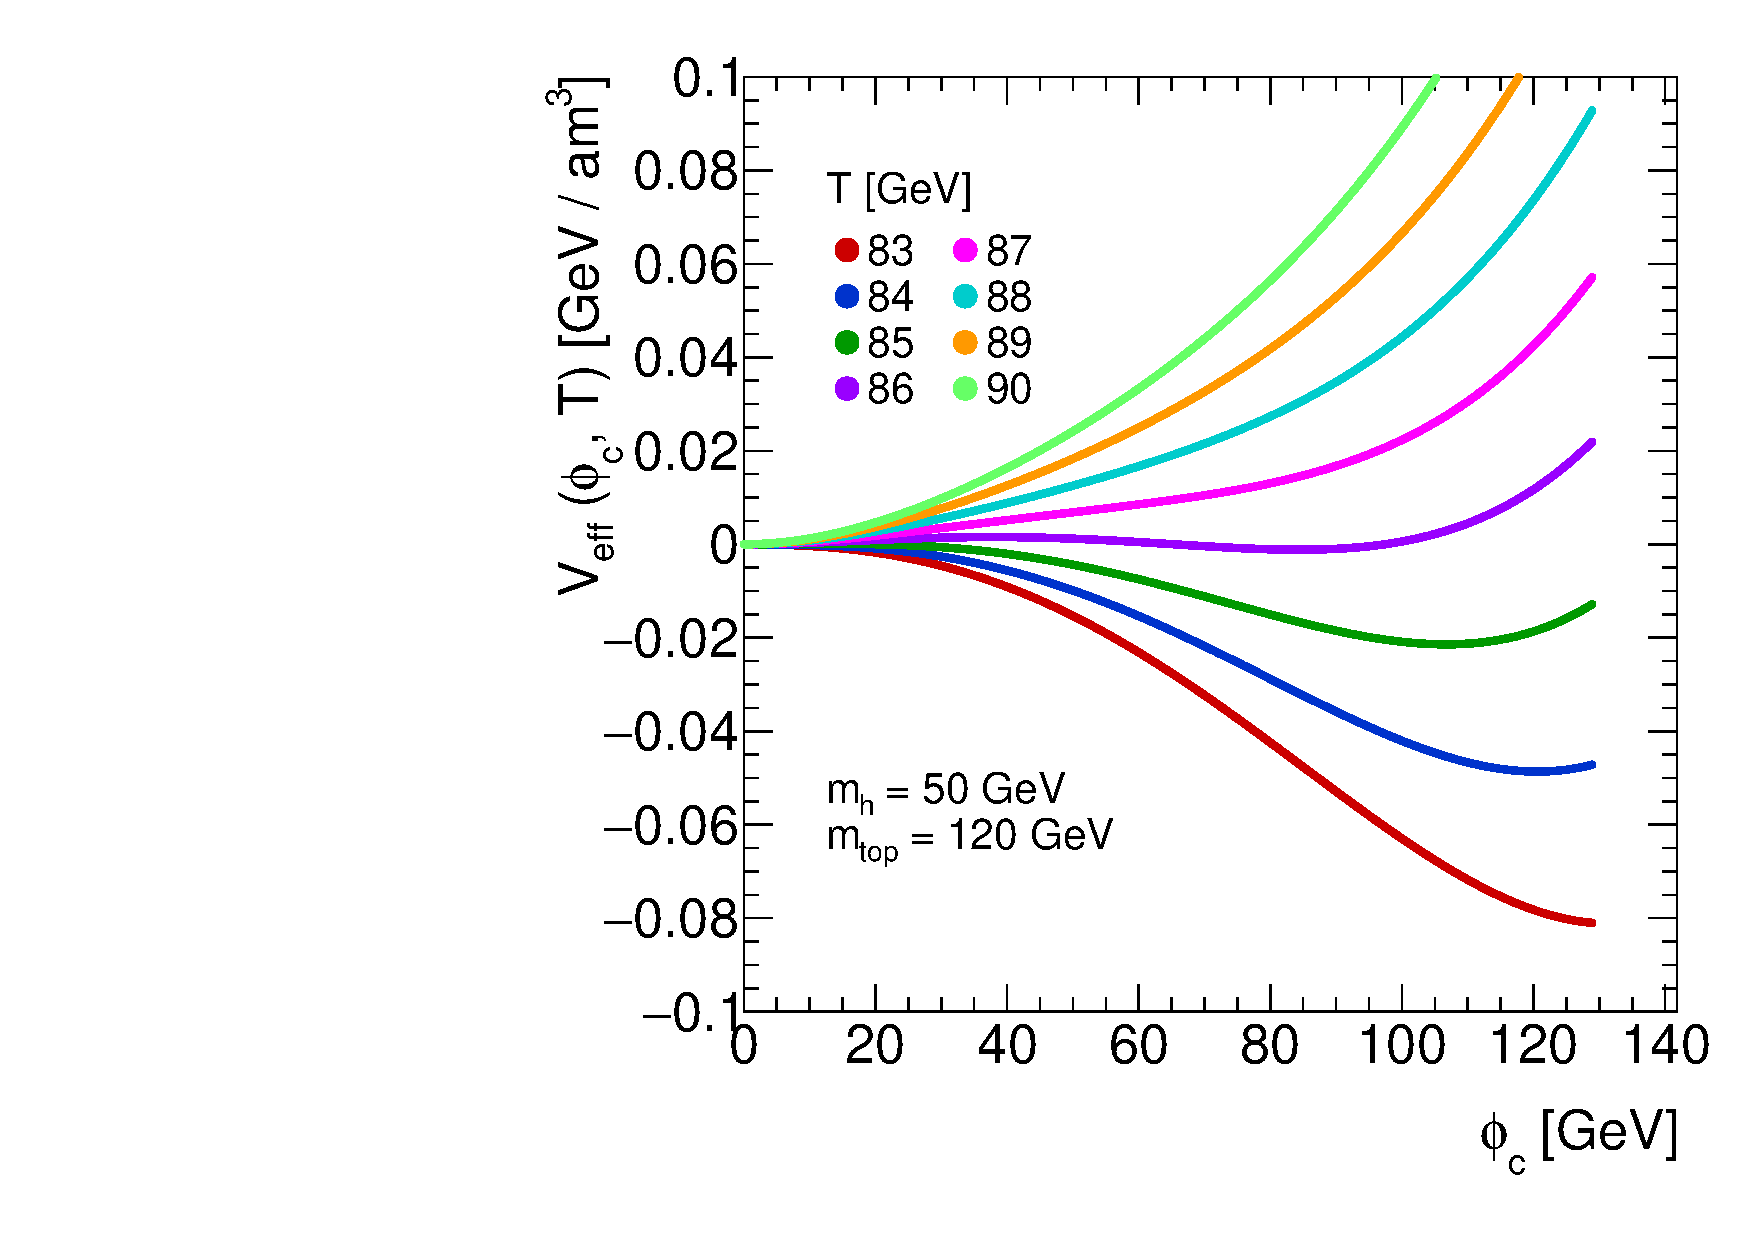
\includegraphics[width=\linewidth]{fopt_effpot.pdf}
    \caption{The effective potential for a fictitious $m_h$ and $m_\text{top}$ is plotted for several different temperatures through the phase transition, exhibiting the emergence of a potential barrier between degenerate local minima. Such a characteristic is indicative of a first order phase transition.}
    \label{fig:fopt}
\end{figure}
As the temperature decreases from $90~\GeV$ we see the development of a secondary minimum around $T\sim86~\GeV$ which becomes a global minimum below that temperature.
This indicates a first order transition, as a local maximum creates a free energy barrier that must be crossed during the phase transition.
At even lower temperatures, the secondary minimum becomes the only minimum, signaling the end of the phase transition.
One key feature we notice in this plot is that the free energy barrier is generally small in comparison to the depth of the minimum at lower temperatures.
In other words, the phase transition appears first order, but is not strongly so.
In Sec.~\ref{sec:baryogenesis} we will quantify this statement more.
Before the Higgs' discovery, numerical estimates that assume a strong first order phase transition put upper bounds on $m_h$; in the literature these range from $m_h < 48~\GeV$ \cite{long12} to $m_h < 77~\GeV$ \cite{gr93}.

Realistically, parameters in the standard model have been measured to have values differing from these toy values.
We now know that $m_h\sim125~\GeV$, well outside these requirements for a strong first-order transition, which explains why the potential barrier appear so weak.
Inputting these measured values to the potential provides the curves shown in Fig.~\ref{fig:sm_effpot}. In particular, the potential barrier (which should be around $T\sim163\GeV$) is no longer visible, indicating that the symmetry restoring phase transition is more likely to be continuous.
\begin{figure}
    \centering
    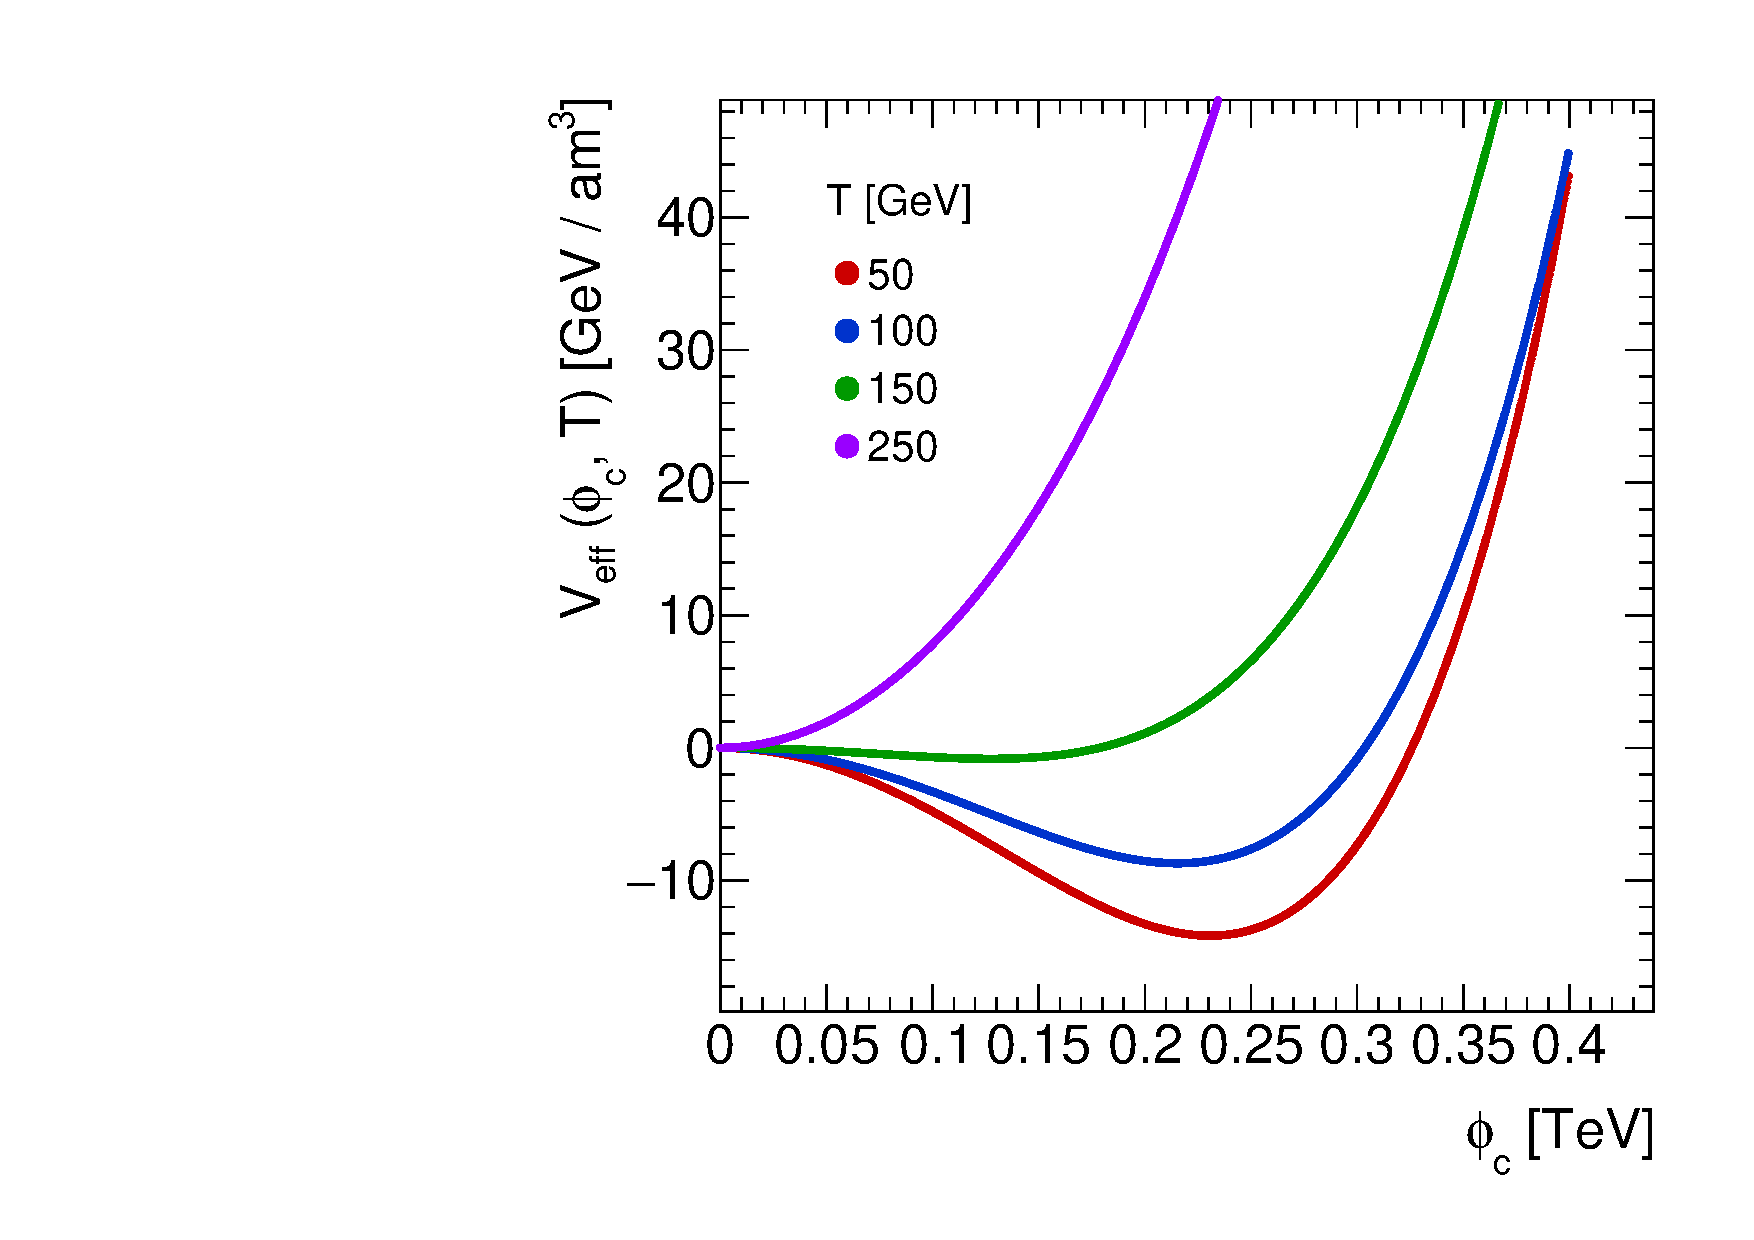
\includegraphics[width=\linewidth]{sm_effpot.pdf}
    \caption{Effective potential in the standard model is plotted for several ambient temperatures as a function of the Higgs' condensate value. Parameters in the effective potential calculated based on measured quantities. Due to the large measured Higgs' mass, the phase transition is expected to be second order.}
    \label{fig:sm_effpot}
\end{figure}

\section{\label{sec:baryogenesis}Implications and Conclusions}
Starting from the tree-level standard model Lagrangian, we have developed a framework in which thermal fluctuations in the Higgs' condensate $\phi_c$ can induce a symmetry restoring phase transition in the electroweak sector.
We demonstrate that the finite temperature Lagrangian theory can be rephrased in terms of a statistical mechanics problem.
The effective potential is calculated to one-loop with contributions from both thermal boson and fermion loops considered.
In particular by coupling $\phi_c$ to gauge bosons we are able to see that the effective boson masses provide a cubic interaction in $\phi_c$, thereby influencing an effective potential barrier.

The strength of the phase transition is of particular importance in cosmology, in the context of baryogenesis.
The matter-antimatter asymmetry we observe remains a pressing issue for cosmology and, under certain conditions, there is some consensus that the spontaneous breaking of the electroweak symmetry at finite temperature provides a natural mechanism for baryogenesis in the very early universe.
The transition from the disordered to ordered state at finite temperature can be understood similarly to a water vapor condensing onto water droplets (``bubbles'') at $100^{\circ}C$.
In the context of electroweak theory, these bubbles can form via ``statistical tunneling'' (a process analogous to quantum tunneling) and are referred to as sphalerons \cite{ah92,long12,quiros99}.
Essentially, a spharelon might be allowed to convert antibaryons/antileptons to baryons/leptons, thus violating baryon number.
However if the phase transition is not first order, the condensate can slowly but continuously vary in magnitude as the temperature decreases, thereby disfavoring sphaleron formation.
This appears to be the case in the standard model with its measured parameters.
More precisely, \cite{long12,kp14} define a ``washout criterion'', under which there can be successful baryogenesis via this mechanism,
\begin{equation}
    \frac{\left<\phi_c(T_c)\right>}{T_c} \gtrsim 0.9-1.
\end{equation}
By visual inspection, we find that for $T_c \approx 163.6~\GeV$, $\left<\phi_c\right> / T_c \sim 0.2-0.3$.
The natural conclusion is that the phase transition is not strongly first order and therefore electroweak baryogenesis is unlikely within the standard model.

Precautions should be taken with these values however.
For example, Coleman and Weinberg \cite{cw73} pointed out that there is a logarithmic singularity in the effective potential at $\phi_c=0$.
At low temperatures, this is irrelevant since $\phi_c$ would prefer to live in the minimum far away from the origin, and we are merely calculating the effect of thermal fluctuations around that minimum in the absence of any particles (namely $W$'s, $Z$'s, $H$'s or top quarks).
More pressing is the relevance of the expansions for the thermal functions $J_{B/F}$, which are only truly valid in the $m/T\ll1$ limit.
We calculated a critical temperature around $163~\GeV$, which is actually a bit less than the top quark mass; as such we are not completely in this limit.
Future theoretical improvement might involve performing a more thorough analysis numerically using the full definitions of $J_{B/F}$.
Although, within this framework the order of the phase transition does not allow successful baryogenesis so it is unclear whether a more accurate study of the critical temperature would change this conclusion.

\bibliographystyle{hplain}
\bibliography{Paper}

\end{document}

% some source links
% 
% https://arxiv.org/pdf/1612.00466.pdf
% https://journals.aps.org/prd/pdf/10.1103/PhysRevD.98.115016
% https://arxiv.org/pdf/hep-ph/9506418.pdf
% https://arxiv.org/pdf/hep-ph/0005272.pdf
% https://arxiv.org/pdf/hep-ph/9608272.pdf
% https://www.sciencedirect.com/science/article/pii/0370269372901098
% https://www.imperial.ac.uk/media/imperial-college/research-centres-and-groups/theoretical-physics/msc/dissertations/2011/Yuhao-Yang-Dissertation.pdf
